% =====================================================================
%  FootBot — Reporte de migración a simulación (ROS 2 + Gazebo)
%  Versión en español. Compilable con pdfLaTeX (Overleaf o TeX Live).
%  El logo de la universidad se incluye automáticamente si existe en
%  src/logo-unet.png (ver portada). Si no, se muestra un placeholder.
% =====================================================================
\documentclass[11pt,a4paper]{article}

% ---------- Idioma y tipografía ----------
\usepackage[utf8]{inputenc}
\usepackage[T1]{fontenc}
\usepackage[spanish,es-tabla]{babel}
\usepackage{lmodern}
\usepackage{microtype}

% ---------- Disposición ----------
\usepackage[a4paper,margin=2.5cm,headheight=15pt]{geometry}
\usepackage{graphicx}
\usepackage{float}
\usepackage{xcolor}
\usepackage{booktabs}
\usepackage{array}
\usepackage{enumitem}
\usepackage{titlesec}
\usepackage{fancyhdr}
\usepackage[most]{tcolorbox}
\usepackage{caption}
\usepackage[document]{ragged2e} % todo el cuerpo alineado a la izquierda (sin justificar)
\usepackage{hyperref}
\usepackage{tikz}
\usetikzlibrary{arrows.meta,positioning}

% ---------- Paleta de color ----------
\definecolor{unetblue}{HTML}{0B3D66}
\definecolor{accent}{HTML}{1B98A0}
\definecolor{softgray}{HTML}{F2F4F7}
\definecolor{darkgray}{HTML}{333333}

\hypersetup{colorlinks=true,linkcolor=unetblue,urlcolor=accent,citecolor=accent,
  pdftitle={FootBot - Migracion a Simulacion ROS 2 + Gazebo},
  pdfauthor={Chacon Gomez Jose Daniel; Castillo Gimenez Alba Patricia}}

\graphicspath{{figures/}{src/}}

% Token de código con guiones bajos literales (sin escapar a mano).
\newcommand{\code}[1]{\texttt{\detokenize{#1}}}

% ---------- Estilo de secciones ----------
\titleformat{\section}{\normalfont\Large\bfseries\color{unetblue}}{\thesection.}{0.5em}{}
\titleformat{\subsection}{\normalfont\large\bfseries\color{accent}}{\thesubsection}{0.5em}{}
\titlespacing*{\section}{0pt}{1.5em}{0.6em}

% ---------- Encabezado / pie ----------
\pagestyle{fancy}
\fancyhf{}
\fancyhead[L]{\footnotesize\color{unetblue}FootBot $\cdot$ Migración a Simulación ROS\,2 + Gazebo}
\fancyhead[R]{\footnotesize\thepage}
\renewcommand{\headrulewidth}{0.4pt}

% ---------- Caja de nota ----------
\newtcolorbox{nota}[1][Nota]{enhanced,breakable,colback=softgray,colframe=accent,
  coltitle=white,fonttitle=\bfseries,title={#1},boxrule=0.6pt,arc=2pt,
  left=7pt,right=7pt,top=5pt,bottom=5pt}

\captionsetup{font=small,labelfont={bf,color=unetblue}}
\captionsetup[figure]{justification=centering}
\setlist{topsep=3pt,itemsep=2pt}

\begin{document}

% ============================ PORTADA ============================
\begin{titlepage}
\centering
\vspace*{0.4cm}

\IfFileExists{src/logo-unet.png}
  {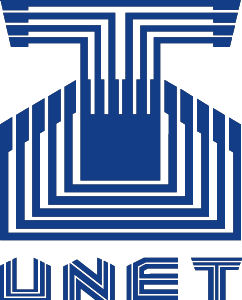
\includegraphics[width=0.18\textwidth]{src/logo-unet.png}\par}
  {\setlength{\fboxsep}{7pt}%
   \fbox{\parbox[c][1.7cm][c]{0.38\textwidth}{\centering\itshape\footnotesize
   Coloque el logo de la universidad en \texttt{src/logo-unet.png}}}\par}

\vspace{1.1cm}
{\scshape\large Universidad Nacional Experimental del Táchira (UNET)\par}
{\scshape\normalsize San Cristóbal, Táchira, Venezuela\par}

\vspace{1.4cm}
\rule{\textwidth}{1.2pt}\par\vspace{0.55cm}
{\huge\bfseries\color{unetblue} De la implementación física a la simulación\par}
\vspace{0.45cm}
{\Large Migración del robot futbolista \textit{FootBot} a un entorno\\[2pt]
ROS\,2 Humble + Gazebo Fortress\par}
\vspace{0.55cm}
\rule{\textwidth}{1.2pt}\par

\vspace{1.3cm}
{\large\bfseries Reporte de entrega — Componente de Simulación\par}

\vspace{2.2cm}
{\large
\renewcommand{\arraystretch}{1.35}
\begin{tabular}{r@{\hskip 1em}l}
\textbf{Autores:} & Chacón Gómez, José Daniel \\
\textbf{Proyecto:} & FootBot / Auto Soccer Bot \\
\textbf{Stack:} & ROS\,2 Humble $\cdot$ Gazebo Fortress \\
\textbf{Fecha:} & Junio de 2026 \\
\end{tabular}\par}

\vfill
\end{titlepage}

% ============================ ÍNDICE (siempre en página propia, tras la portada) ============================
\clearpage
{\hypersetup{linkcolor=darkgray}\tableofcontents}
\thispagestyle{fancy}
\clearpage

% ============================ RESUMEN ============================
\section*{Resumen}
\addcontentsline{toc}{section}{Resumen}

El proyecto \textit{FootBot} (también llamado \textit{Auto Soccer Bot}) nació como
un robot futbolista físico de bajo costo, construido alrededor de un ESP32\mbox{-}CAM,
con la percepción y la toma de decisiones ejecutándose en un portátil. Este reporte
documenta la \textbf{migración de ese sistema hacia un entorno de simulación} basado
en \textbf{ROS\,2 Humble} y \textbf{Gazebo Fortress}. Se explica \emph{qué} se construyó,
\emph{por qué} se decidió pasar del hardware real a la simulación, \emph{cómo} se trasladó
cada componente del robot físico a su equivalente simulado, y \emph{qué fases} se ejecutaron:
fundamentos (modelo del robot y mundos), puentes de control, percepción simulada,
comportamientos autónomos deterministas (\emph{Control de balón} y \emph{Llegar a la portería})
y la tubería de \emph{datasets} y entrenamiento de visión. El resultado es un \emph{workspace}
de ROS\,2 reproducible que conserva la compatibilidad con el robot ESP32 como referencia,
a la vez que habilita el desarrollo seguro, repetible y escalable de comportamientos de
fútbol robótico.

\medskip
\noindent\textbf{Palabras clave:} robótica móvil, ROS\,2 Humble, Gazebo Fortress, simulación,
máquinas de estados finitos, percepción, YOLO, fútbol robótico.

% ============================ 1. INTRODUCCIÓN ============================
\section{Introducción}
\label{sec:intro}

El sistema original, \textit{Auto Soccer Bot}, es un robot móvil de tracción diferencial
basado en un ESP32\mbox{-}CAM que opera en dos modos complementarios: (i) \textbf{control manual}
mediante gestos de la mano detectados por visión (MediaPipe) en un portátil, y
(ii) \textbf{modo automático}, en el que el ESP32\mbox{-}CAM transmite vídeo por Wi\mbox{-}Fi a una
aplicación en el host que realiza detección del balón (umbrales HSV junto con YOLO) y alimenta
una máquina de estados finitos (FSM) para seguir el balón. Todos los comandos viajan por una
API HTTP (\code{/move}) desacoplada del flujo de vídeo.

Ese diseño valida la arquitectura distribuida (percepción pesada en el portátil, actuación en
tiempo real en el robot), pero arrastra las limitaciones propias de cualquier banco de pruebas
físico: dependencia del hardware, de la iluminación y de un único robot, fragilidad mecánica,
y ciclos de iteración lentos. Para avanzar hacia comportamientos de fútbol más ambiciosos
—posesión del balón, conducción hacia portería, oponentes y juego en equipo— se decidió
construir una \textbf{capa de simulación} sobre ROS\,2 y Gazebo.

Este documento reporta esa migración. La capa de simulación vive aislada bajo el directorio
\code{/simulation} y mantiene intactas las aplicaciones ESP32 y Python originales como referencia.
El resto del reporte se organiza así: la Sección~\ref{sec:motivacion} expone la motivación;
la Sección~\ref{sec:mapeo} describe cómo se trasladó cada componente físico a su equivalente
simulado; la Sección~\ref{sec:arquitectura} presenta la arquitectura del sistema de simulación;
la Sección~\ref{sec:fases} detalla las fases ejecutadas; las Secciones~\ref{sec:comportamientos}
y~\ref{sec:percepcion} profundizan en los comportamientos autónomos y en la percepción;
la Sección~\ref{sec:resultados} resume el estado actual y la Sección~\ref{sec:futuro} el trabajo futuro.

\begin{figure}[H]
\centering
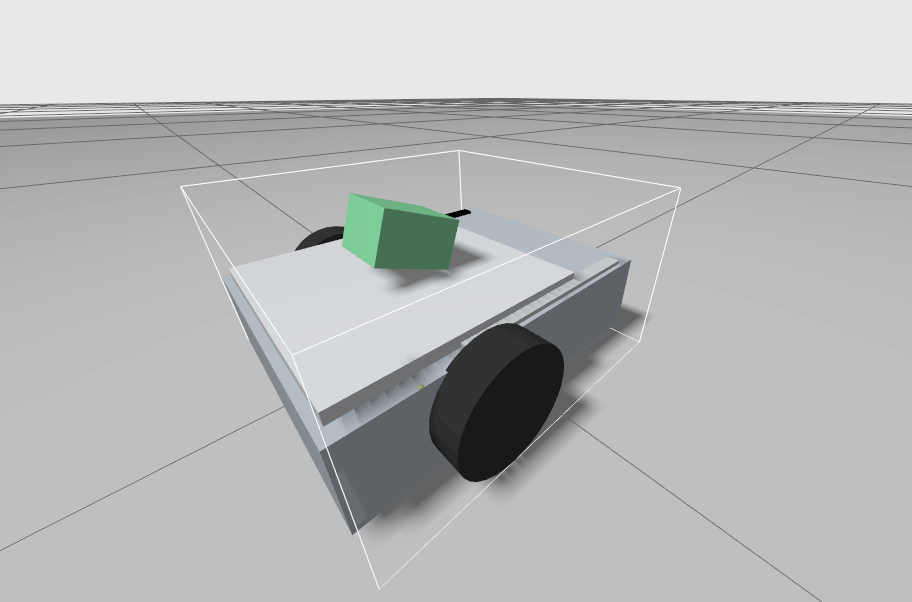
\includegraphics[width=0.86\textwidth]{figures/simulation-overview.png}
\caption{FootBot generado en Gazebo con la cámara simulada del robot, la iluminación y los
objetos de validación visibles. La simulación reproduce el robot y su sensor de cámara dentro
de un mundo controlado y repetible.}
\label{fig:overview}
\end{figure}

\subsection{¿Qué son ROS\,2 y Gazebo?}
\textbf{ROS\,2} (\emph{Robot Operating System 2}) no es un sistema operativo, sino un \emph{middleware}
de robótica: un conjunto de librerías y convenciones para construir el sistema como un grafo de procesos
independientes —los \emph{nodos}— que se comunican publicando y suscribiéndose a canales con nombre, los
\emph{topics}. Aporta mensajes tipados, parámetros, lanzamiento coordinado y descubrimiento automático,
lo que favorece un diseño modular y reutilizable.

\textbf{Gazebo} (edición \emph{Fortress}) es un \emph{simulador} de robótica 3D: modela física
(gravedad, colisiones, fricción), sensores (cámaras, odometría) y mundos completos, y permite generar
(\emph{spawn}) un robot para observar su comportamiento sin hardware. La pieza que une ambos mundos es
el \code{ros_gz_bridge}, que traduce los datos entre Gazebo y los \emph{topics} de ROS\,2; gracias a él,
los nodos de percepción y control operan igual frente a un robot real o uno simulado.

\subsection{Continuidad con el trabajo previo}
Este trabajo da continuidad al reporte anterior del \emph{Auto Soccer Bot}, centrado en el robot físico
ESP32\mbox{-}CAM de control híbrido. Aquel sistema ya logró: (i) teleoperación manual por gestos de la
mano (MediaPipe); (ii) un modo automático de \textbf{seguimiento del balón} con percepción híbrida
HSV+YOLO y una FSM; y (iii) el entrenamiento y validación de detectores YOLO de \code{goal} y
\code{opponent} (mAP@0.5 = 0.991). Sin embargo, esos detectores de portería y oponente \textbf{no
llegaron a integrarse} en la FSM del modo automático: la fusión de decisiones multiobjeto quedó
explícitamente como trabajo futuro.

¿Qué cambió de forma notable al pasar a la simulación?
\begin{itemize}
  \item \textbf{Plataforma.} Del robot ESP32\mbox{-}CAM físico a un FootBot simulado en Gazebo (modelo
  URDF de tracción diferencial); el \emph{stream} MJPEG pasa a ser un \emph{topic} de cámara.
  \item \textbf{Comunicación y latencia.} Del enlace Wi\mbox{-}Fi/HTTP —sensible a la latencia, que
  obligaba a retención del último frame y a limitar la tasa de comandos— a \emph{topics} de ROS\,2 en un
  grafo local, con latencia mucho menor y estable (Sección~\ref{sec:motivacion}).
  \item \textbf{La portería, por fin integrada.} El comportamiento \emph{Llegar a la portería} fusiona
  \code{ball}\,+\,\code{goal} en el lazo percepción$\to$decisión y conduce el balón a la portería: la
  fusión multiobjeto que el reporte previo dejaba pendiente \textbf{ya está parcialmente realizada}
  (resta el oponente).
  \item \textbf{Ingeniería.} De aplicaciones monolíticas en el host a \textbf{paquetes ROS\,2 modulares},
  con un patrón determinista percepción$\to$estado$\to$FSM, una suite de pruebas y un \emph{árbitro} de
  simulación para puntuar goles.
\end{itemize}

% ============================ 2. MOTIVACIÓN ============================
\section{Motivación: ¿por qué migrar a simulación?}
\label{sec:motivacion}

La migración a un entorno simulado no busca reemplazar al robot físico, sino crear un banco de
pruebas donde la lógica de fútbol pueda desarrollarse y validarse de forma \textbf{rápida, segura
y reproducible}. Las razones principales fueron:

\begin{itemize}
  \item \textbf{Reproducibilidad y determinismo.} Cada escenario (posición del balón, de la portería,
  del robot) se reinicia idéntico, lo que permite comparar cambios de comportamiento sin el ruido
  del mundo físico.
  \item \textbf{Seguridad y costo.} No hay motores que quemar, baterías que agotar ni colisiones que
  reparar; iterar es gratis y no desgasta hardware.
  \item \textbf{Velocidad de iteración.} No es necesario montar el robot ni el campo físico para probar
  una idea: se lanza un \emph{world} y se ejecuta el comportamiento.
  \item \textbf{Escenarios paralelos y casos límite.} La simulación permite ejecutar varios escenarios
  aislados a la vez (p.\,ej., balón al frente, lejos y detrás) en un mismo mundo, algo inviable con un
  solo robot real.
  \item \textbf{Independencia del hardware y la iluminación.} La cámara simulada entrega imágenes
  consistentes, eliminando la fragilidad del detector frente a cambios de luz que afectaba al lazo físico.
  \item \textbf{Latencia menor y estable.} En el robot físico, el enlace Wi\mbox{-}Fi/HTTP entre el
  portátil y el ESP32 añadía un retardo variable al lazo de control; en simulación, la comunicación por
  \emph{topics} locales reduce y estabiliza esa latencia.
  \item \textbf{Base para comportamientos avanzados.} Posesión del balón y conducción hacia portería
  requieren muchísimas repeticiones; la simulación las hace prácticas.
  \item \textbf{Continuidad.} El trabajo previo no se descarta: el robot ESP32 y sus apps Python quedan
  como referencia, y un puente mantiene la compatibilidad del antiguo protocolo HTTP \code{/move}.
\end{itemize}

\begin{nota}[Latencia y compatibilidad HTTP]
Una limitación importante del montaje físico era la \textbf{latencia variable del enlace Wi\mbox{-}Fi}
entre el portátil y el ESP32: tanto el vídeo como los comandos viajaban por HTTP, lo que introducía
retardo y obligaba a paliativos como la retención del último frame y la limitación de la tasa de
comandos (el robot llegaba a \emph{perseguir el pasado}). En la simulación, la comunicación ocurre por
\emph{topics} de ROS\,2 dentro de un mismo grafo local, de modo que esa latencia se \textbf{reduce
drásticamente y se estabiliza}.

¿Conservamos el modo de operar por HTTP? \textbf{Sí, pero solo por compatibilidad}: el paquete
\code{footbot_bridge} mantiene vivo el antiguo endpoint HTTP \code{/move} traduciéndolo a \code{/cmd_vel}.
El control nativo y recomendado dentro de la simulación es directamente por el \emph{topic} \code{/cmd_vel}.
\end{nota}

\begin{nota}[Regla de oro del control]
En cualquier modo de lanzamiento, \textbf{un solo nodo} debe ser dueño de \code{/cmd_vel} a la vez.
Esta regla, heredada del diseño original, evita que controladores en competencia se peleen por el
robot y es un principio transversal de toda la arquitectura de simulación.
\end{nota}

% ============================ 3. MAPEO FÍSICO -> SIMULACIÓN ============================
\section{Del robot físico al entorno simulado}
\label{sec:mapeo}

La estrategia fue \emph{simulation\mbox{-}first}: en lugar de portar el firmware del ESP32, se
reconstruyó cada capacidad del robot como uno o varios paquetes de ROS\,2, reutilizando los
conceptos (tracción diferencial, cámara, detección de balón, FSM) pero apoyándose en la
infraestructura nativa de ROS y Gazebo. La Tabla~\ref{tab:mapeo} resume la correspondencia.

\renewcommand{\arraystretch}{1.3}
\begin{table}[H]
\caption{Correspondencia entre el robot físico y su equivalente simulado.}
\label{tab:mapeo}
\raggedright
\small
\begin{tabular}{>{\raggedright\arraybackslash}p{0.43\linewidth} >{\raggedright\arraybackslash}p{0.5\linewidth}}
\toprule
\textbf{Componente del robot físico} & \textbf{Equivalente en simulación (ROS\,2 + Gazebo)} \\
\midrule
Chasis y tracción diferencial (motores DC, driver L298N) & Modelo URDF/Xacro (\code{footbot_description}) accionado por el plugin DiffDrive de Gazebo (\code{footbot_gazebo}) \\
Cámara ESP32\mbox{-}CAM (stream MJPEG por Wi\mbox{-}Fi) & Cámara simulada de Gazebo, puenteada a \code{/camera/image_raw} por \code{ros_gz_bridge} \\
API HTTP \code{/move} del firmware ESP32 & Puente \code{footbot_bridge} (HTTP \code{/move} $\rightarrow$ \code{/cmd_vel}) y control nativo por \code{/cmd_vel} \\
Control manual por gestos (MediaPipe en el host) & \code{footbot_perception} (detección de manos) + \code{footbot_control} (\code{gesture_to_cmd_vel}) \\
Detección de balón por color HSV (host) & \code{footbot_perception} (\code{ball_detector}) \\
Modelos YOLO de portería/oponente (\code{soccer_vision}) & \code{footbot_soccer_vision} (detectores YOLO, captura y herramientas de \emph{dataset}) \\
FSM de seguimiento de balón (host) & \code{footbot_soccer_behavior} (\code{ball_control_fsm}, \code{reach_goal_fsm}, estimadores de estado y \emph{skills}) \\
Archivos de configuración de Python & Parámetros de ROS en archivos YAML \\
Red Wi\mbox{-}Fi local (host $\leftrightarrow$ robot) & Topics de ROS\,2 dentro del grafo de nodos \\
\bottomrule
\end{tabular}
\end{table}

En esencia: lo que antes era un \emph{stream} MJPEG hacia un detector y un \texttt{POST} HTTP hacia el
firmware, ahora es un \emph{topic} de cámara hacia un nodo de percepción y un \emph{topic} \code{/cmd_vel}
hacia el robot simulado. El antiguo protocolo \code{/move} no se abandona: el paquete
\code{footbot_bridge} lo traduce a \code{/cmd_vel}, conservando compatibilidad con el ecosistema ESP32.

% ============================ 4. ARQUITECTURA ============================
\section{Arquitectura del sistema de simulación}
\label{sec:arquitectura}

\subsection{Stack tecnológico}
El entorno soportado es deliberadamente el oficial y de bajo riesgo para Ubuntu~22.04:

\begin{itemize}
  \item \textbf{ROS\,2 Humble Hawksbill} como middleware de robótica.
  \item \textbf{Gazebo Fortress} como simulador físico/visual.
  \item \textbf{\code{ros-humble-ros-gz}} como integración oficial ROS\,$\leftrightarrow$\,Gazebo.
  \item \textbf{Ubuntu 22.04 (jammy)} y \textbf{Python 3.10}.
\end{itemize}

Se descartó ROS\,2 Jazzy/Gazebo Harmonic en este host porque apuntan a Ubuntu~24.04; mantener el
emparejamiento por defecto reduce el riesgo y evita soluciones alternativas de versión.

\subsection{Paquetes del \emph{workspace}}
El \emph{workspace} de ROS\,2 vive en \code{simulation/ros2_ws/} y se divide en paquetes con
responsabilidades acotadas (Tabla~\ref{tab:paquetes}).

\renewcommand{\arraystretch}{1.25}
\begin{table}[H]
\caption{Paquetes del \emph{workspace} de simulación y su responsabilidad.}
\label{tab:paquetes}
\raggedright
\small
\begin{tabular}{>{\raggedright\arraybackslash}p{0.30\linewidth} l >{\raggedright\arraybackslash}p{0.40\linewidth}}
\toprule
\textbf{Paquete} & \textbf{Tipo} & \textbf{Responsabilidad} \\
\midrule
\code{footbot_common} & ament\_python & Constantes compartidas (topics, frames, geometría, utilidades). \\
\code{footbot_description} & ament\_cmake & Modelo Xacro del robot, frames, ruedas, cámara, RViz. \\
\code{footbot_gazebo} & ament\_cmake & Mundos, modelos, configuración del puente, plugin de arrastre del balón. \\
\code{footbot_bringup} & ament\_cmake & Orquestación de lanzamiento de todos los modos. \\
\code{footbot_bridge} & ament\_python & Puente HTTP \code{/move} (compatible ESP32) hacia \code{/cmd_vel}. \\
\code{footbot_perception} & ament\_python & Webcam, detección de manos, detección HSV del balón, visor de depuración. \\
\code{footbot_control} & ament\_python & Controladores gesto\,$\to$\,velocidad y seguidor de balón simple. \\
\code{footbot_soccer_msgs} & ament\_cmake & Mensajes propios (\code{BallState}, \code{BallGoalState}). \\
\code{footbot_soccer_behavior} & ament\_python & Estimación de estado, \emph{skills} y FSM de los comportamientos. \\
\code{footbot_soccer_vision} & ament\_python & Percepción YOLO, captura y herramientas de \emph{dataset}. \\
\bottomrule
\end{tabular}
\end{table}

\subsection{Flujo de datos}
El patrón general es: Gazebo publica sensores (cámara, odometría) por Gazebo Transport, el
\code{ros_gz_bridge} los traduce a topics de ROS, los nodos de percepción producen detecciones,
los estimadores las convierten en estado, y las FSM deciden y publican \code{/cmd_vel}
(Fig.~\ref{fig:arch}).

\begin{figure}[H]
\centering
\resizebox{\textwidth}{!}{%
\begin{tikzpicture}[
  every node/.style={font=\footnotesize},
  box/.style={draw=unetblue, line width=0.7pt, rounded corners=2pt, fill=softgray,
              minimum width=26mm, minimum height=13mm, align=center, text width=24mm},
  gz/.style ={box, fill=unetblue!12},
  per/.style={box, draw=accent, fill=accent!15},
  beh/.style={box, fill=unetblue!10},
  ar/.style ={-{Stealth[length=2mm]}, line width=0.8pt, draw=darkgray},
  tl/.style ={font=\scriptsize\ttfamily, fill=white, inner sep=1.5pt}
]
  \node[gz]  (gz) {Gazebo\\[-1pt]{\scriptsize mundo + robot}};
  \node[box, right=28mm of gz] (br) {ros\_gz\_bridge};
  \node[per, right=12mm of br] (pe) {Percepción\\[-1pt]{\scriptsize ball\_detector / yolo\_detector}};
  \node[per, right=26mm of pe] (es) {Estimador\\[-1pt]{\scriptsize de estado}};
  \node[beh, right=30mm of es] (fs) {FSM\\[-1pt]{\scriptsize ball\_control\_fsm / reach\_goal\_fsm}};
  \draw[ar] (gz) -- (br) node[tl,midway,above]{/camera/image\_raw};
  \draw[ar] (br) -- (pe);
  \draw[ar] (pe) -- (es) node[tl,midway,above]{/ball\_detection};
  \draw[ar] (es) -- (fs) node[tl,midway,above]{/soccer/ball\_state};
  \draw[ar] (fs.south) -- ++(0,-9mm) -| (gz.south);
  \path (fs.south) -- (gz.south) node[tl,midway,yshift=-9mm]{/cmd\_vel};
\end{tikzpicture}}
\caption{Arquitectura abstracta y flujo de \emph{topics}: Gazebo entrega la imagen de la cámara, el
puente la traduce a ROS, la percepción detecta, el estimador produce el estado y la FSM cierra el lazo
publicando \texttt{/cmd\_vel}. Se muestran solo los \emph{topics} principales.}
\label{fig:arch}
\end{figure}

\begin{nota}[Tubería de \emph{Control de balón}]
\code{/camera/image_raw} $\rightarrow$ \code{ball_detector} $\rightarrow$ \code{/ball_detection}
$\rightarrow$ \code{ball_state_estimator} $\rightarrow$ \code{/soccer/ball_state}
$\rightarrow$ \code{ball_control_fsm} $\rightarrow$ \code{/cmd_vel}
\end{nota}

\begin{nota}[Tubería de \emph{Llegar a la portería}]
\code{/camera/image_raw} $\rightarrow$ \code{yolo_detector} $\rightarrow$ \code{/soccer/detections}
$\rightarrow$ \code{ball_goal_state_estimator} $\rightarrow$ \code{/soccer/ball_goal_state}
$\rightarrow$ \code{reach_goal_fsm} $\rightarrow$ \code{/cmd_vel}
\end{nota}

% ============================ 5. FASES ============================
\section{Fases del trabajo realizado}
\label{sec:fases}

\subsection{Fase 1 — Fundamentos: modelo, mundos y arranque}
Se decidió el \emph{stack} (ROS\,2 Humble + Gazebo Fortress), se creó el \emph{workspace} de
\emph{colcon}, y se construyó el modelo del robot en Xacro (\code{footbot_description}): chasis,
ruedas, rueda loca, sensor de cámara y frames (\code{base_footprint}, \code{base_link},
\code{camera_link}, etc.). Se prepararon los mundos de Gazebo y el lanzamiento base, que genera
(\emph{spawn}) el robot y puentea \code{/cmd_vel}, \code{/odom} y los topics de cámara.

\subsection{Fase 2 — Puentes de control}
Se habilitaron las tres vías de control: comandos directos por \code{/cmd_vel}; el puente
\code{footbot_bridge}, que mantiene el antiguo endpoint HTTP \code{/move} del ESP32 traduciéndolo a
\code{/cmd_vel}; y el control por gestos nativo de ROS, que usa la webcam y MediaPipe para producir
\code{gesture_to_cmd_vel}. Siempre bajo la regla de un único dueño de \code{/cmd_vel}.

\subsection{Fase 3 — Percepción simulada}
La cámara simulada del robot publica en \code{/camera/image_raw}. Sobre ella se portó la detección
de balón por color (\code{ball_detector} en \code{footbot_perception}), determinista y ajustada al
balón naranja simulado, y se incorporó la visión de fútbol con YOLO en \code{footbot_soccer_vision}.

\subsection{Fase 4 — Comportamientos autónomos deterministas}
Es el corazón del trabajo: dos comportamientos de fútbol construidos sobre el patrón
\emph{percepción $\rightarrow$ estimador de estado $\rightarrow$ FSM $\rightarrow$ un único dueño de}
\code{/cmd_vel}. Se detallan en la Sección~\ref{sec:comportamientos}.

\subsection{Fase 5 — Datasets y entrenamiento de visión}
Se construyó la tubería completa de datos para YOLO: captura de imágenes desde la escena
(\code{image_capture}), etiquetado en Label Studio, aumento conservador del \emph{dataset},
preparación y validación de las particiones, y entrenamiento/evaluación del detector de
\code{ball} + \code{goal}. Se detalla en la Sección~\ref{sec:percepcion}.

\subsection{Mundos y escenarios}
Se crearon mundos para cada necesidad: pruebas de cámara, control de balón de un escenario,
prueba multi\mbox{-}carril (tres escenarios aislados en un mismo mundo), escena de \emph{Llegar a la
portería} (robot + balón dinámico + portería) y el campo de fútbol completo con paredes, porterías,
balón central y equipos en espejo (Fig.~\ref{fig:field}).

% ============================ 6. COMPORTAMIENTOS ============================
\section{Comportamientos autónomos en detalle}
\label{sec:comportamientos}

Ambos comportamientos comparten una filosofía \textbf{determinista}: la percepción alimenta a un
estimador de estado, el estimador alimenta a una FSM, y exactamente un controlador es dueño de
\code{/cmd_vel}. Las \emph{skills} sólo producen comandos \code{Twist} acotados para el estado actual;
la FSM es la única dueña de las transiciones.

\subsection{Control de balón (Ball Control)}
Es el primer comportamiento autónomo: encontrar, aproximarse, hacer contacto y mantener el balón
naranja en una zona de control frontal (Fig.~\ref{fig:ballcontrol}). El detector HSV produce
\code{/ball_detection}; el \code{ball_state_estimator} convierte la detección \code{Detection2D} en un
\code{BallState}; y el \code{ball_control_fsm} recorre estados como \code{SEARCH_BALL},
\code{ALIGN_TO_BALL}, \code{APPROACH_BALL}, \code{CONTACT_BALL}, \code{CONTROL_BALL},
\code{ROTATE_WITH_BALL}, \code{RECOVER_BALL} y \code{STOP_SAFE}. El estimador usa el radio aparente del
balón y el campo de visión de la cámara para estimar un rango aproximado: apropiado para simulación,
sin pretender ser un estimador de pose 3D calibrado.

\begin{figure}[H]
\centering
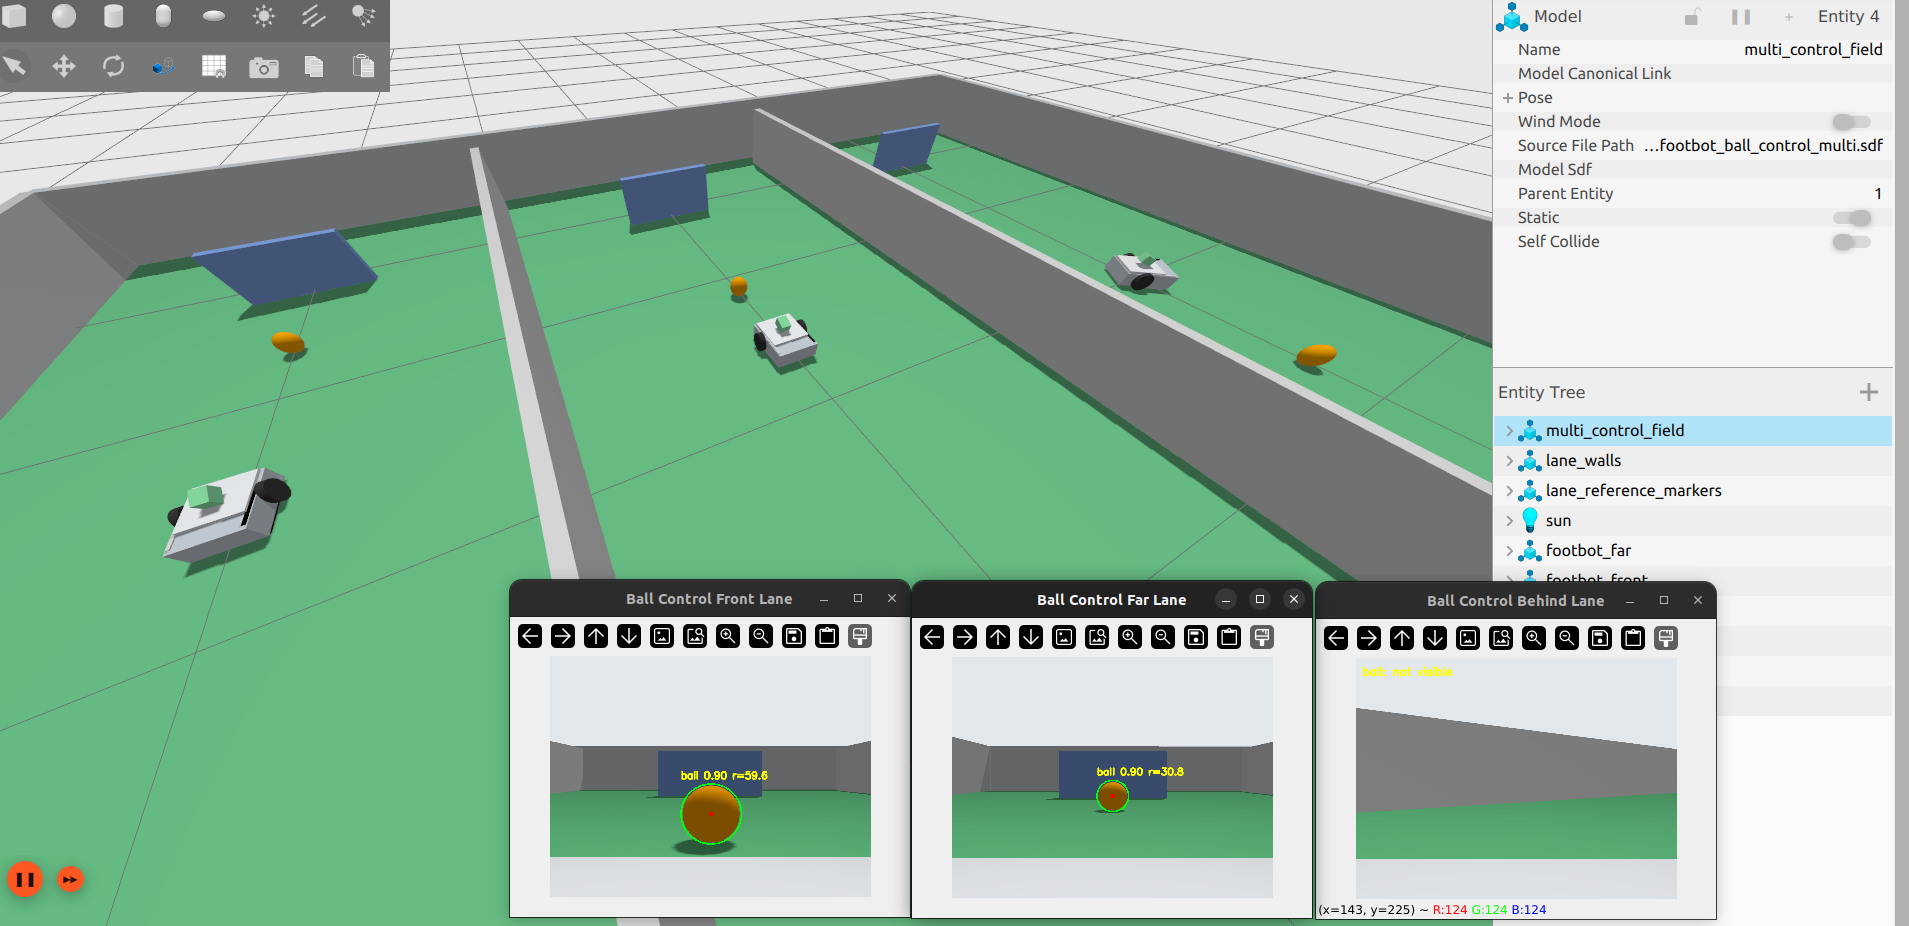
\includegraphics[width=0.78\textwidth]{figures/ball-control-debug.png}
\caption{Comportamiento de Control de balón ejecutándose en Gazebo, con el visor de depuración que
muestra el balón naranja detectado y la realimentación de estado.}
\label{fig:ballcontrol}
\end{figure}

\subsection{Llegar a la portería (Reach Goal)}
Es el comportamiento de producción: empujar el balón hacia una portería visible usando la cámara del
robot. Un detector YOLO de \code{ball} + \code{goal} publica \code{/soccer/detections}; el
\code{ball_goal_state_estimator} produce un \code{BallGoalState} derivado únicamente de la imagen; y el
\code{reach_goal_fsm} es el único dueño de \code{/cmd_vel}. Cada decisión de control está guiada por la
percepción: el comportamiento \textbf{nunca} lee las poses reales (\emph{ground truth}) de Gazebo para
navegar. La Tabla~\ref{tab:reachstates} resume sus estados.

\renewcommand{\arraystretch}{1.2}
\begin{table}[H]
\caption{Estados de la FSM de \emph{Llegar a la portería}.}
\label{tab:reachstates}
\raggedright
\small
\begin{tabular}{l >{\raggedright\arraybackslash}p{0.62\linewidth}}
\toprule
\textbf{Estado} & \textbf{Descripción} \\
\midrule
\code{SEARCH_BALL} & Sin balón a la vista; rota para escanear. \\
\code{APPROACH_BALL} & Balón visible; conduce hacia él (frena al crecer). \\
\code{CONTROL_BALL} & Balón en la zona de control frontal; lo mantiene centrado. \\
\code{SEARCH_GOAL} & Balón controlado, portería no vista; rota sosteniendo el balón. \\
\code{ALIGN_BALL_TO_GOAL} & Balón y portería visibles pero desalineados; gira suave con el balón. \\
\code{DRIBBLE_TO_GOAL} & Balón alineado con la portería; avanza. \\
\code{COMMIT_TO_GOAL} & Respaldo a corta distancia; empuja despacio sólo centrando el balón. \\
\code{RECOVER_BALL} & Control perdido; retrocede y readquiere el balón. \\
\code{STOP_SAFE} & Percepción obsoleta o parada de emergencia; velocidad cero. \\
\code{GOAL_SCORED} & El árbitro de simulación detectó gol; velocidad cero permanente. \\
\bottomrule
\end{tabular}
\end{table}

\begin{figure}[H]
\centering
\resizebox{\textwidth}{!}{%
\begin{tikzpicture}[
  >={Stealth[length=2mm]},
  st/.style={draw, rounded corners=2pt, line width=0.7pt, fill=softgray,
             minimum width=22mm, minimum height=8mm, inner sep=2pt,
             font=\scriptsize\ttfamily, align=center},
  main/.style={st, draw=unetblue, fill=unetblue!10},
  goal/.style={st, draw=accent, line width=1pt, fill=accent!20},
  exc/.style ={st, draw=darkgray, fill=white},
  e/.style={->, line width=0.7pt, draw=unetblue},
  d/.style={->, line width=0.6pt, draw=darkgray, densely dashed},
  lbl/.style={font=\tiny, fill=white, inner sep=1pt}
]
  % fila superior (camino principal)
  \node[main] (sb) at (0,0)    {SEARCH\_BALL};
  \node[main] (ab) at (3.8,0)  {APPROACH\_BALL};
  \node[main] (cb) at (7.6,0)  {CONTROL\_BALL};
  \node[main] (sg) at (11.4,0) {SEARCH\_GOAL};
  % fila inferior (regreso)
  \node[main] (al) at (11.4,-2){ALIGN\_BALL\_TO\_GOAL};
  \node[main] (dr) at (7.6,-2) {DRIBBLE\_TO\_GOAL};
  \node[main] (co) at (3.8,-2) {COMMIT\_TO\_GOAL};
  \node[goal] (gs) at (0,-2)   {GOAL\_SCORED};
  % estados de excepción
  \node[exc] (rb) at (5.7,-3.9){RECOVER\_BALL};
  \node[exc] (ss) at (9.5,-3.9){STOP\_SAFE};
  % camino principal
  \draw[e] (sb) -- (ab);
  \draw[e] (ab) -- (cb);
  \draw[e] (cb) -- (sg);
  \draw[e] (sg) -- (al);
  \draw[e] (al) -- (dr);
  \draw[e] (dr) -- (co);
  \draw[e] (co) -- (gs);
  % excepciones (discontinuo)
  \draw[d] (dr) -- (rb) node[lbl,midway,right]{pierde control};
  \draw[d] (al) -- (ss) node[lbl,midway,right]{percep. obsoleta};
\end{tikzpicture}}
\caption{Esquema de la FSM de \emph{Llegar a la portería}. En azul, el camino principal (de buscar el
balón a marcar, con \texttt{GOAL\_SCORED} resaltado como estado terminal); en líneas discontinuas, las
salidas de recuperación y de seguridad. Cualquier estado de posesión puede caer a \texttt{RECOVER\_BALL}
al perder el control, y la percepción obsoleta fuerza \texttt{STOP\_SAFE}; ambos retoman la búsqueda al
recuperarse.}
\label{fig:fsm}
\end{figure}

La Figura~\ref{fig:fsm} resume gráficamente estas transiciones. Dos mecanismos hacen robusto el comportamiento. Primero, una \textbf{memoria temporal de la portería}:
cuando el robot se acerca a la boca y la portería desaparece del cuadro, el estimador reutiliza
brevemente la última orientación válida, evitando recaer en \code{SEARCH_GOAL} por una pérdida puntual
de YOLO. Segundo, el estado \code{COMMIT_TO_GOAL}, un respaldo \emph{sin reentrenamiento} que, tras
\code{DRIBBLE_TO_GOAL}, mantiene un empuje lento centrado en el balón hasta que el árbitro reporta el gol.

\begin{nota}[Detección de gol = lógica de árbitro, no percepción del robot]
La puntuación usa un monitor de simulación (\code{reach_goal_score_monitor}) que observa el \emph{stream}
de poses del mundo de Gazebo y publica \code{/soccer/goal_scored} cuando el balón permanece dentro de la
zona de gol el tiempo suficiente. Esto permite \textbf{detener} el episodio limpiamente tras un gol
\textbf{sin} dar al robot información privilegiada para navegar.
\end{nota}

% ============================ 7. PERCEPCIÓN Y DATASETS ============================
\section{Percepción y \emph{datasets}}
\label{sec:percepcion}

\subsection{Cámaras y detección}
La cámara simulada del robot publica en \code{/camera/image_raw} (y \code{/camera/camera_info}); el campo
de fútbol añade además una cámara cenital en \code{/soccer/camera/image_raw}. Sobre estas imágenes operan
dos familias de detectores: el detector HSV determinista del balón (\code{ball_detector}) y los detectores
YOLO de \code{footbot_soccer_vision}, que emiten \code{vision_msgs/Detection2DArray}.

El control por gestos, heredado del modo manual del robot real, también se reprodujo de forma nativa en ROS
con MediaPipe (Fig.~\ref{fig:gesture}).

\begin{figure}[H]
\centering
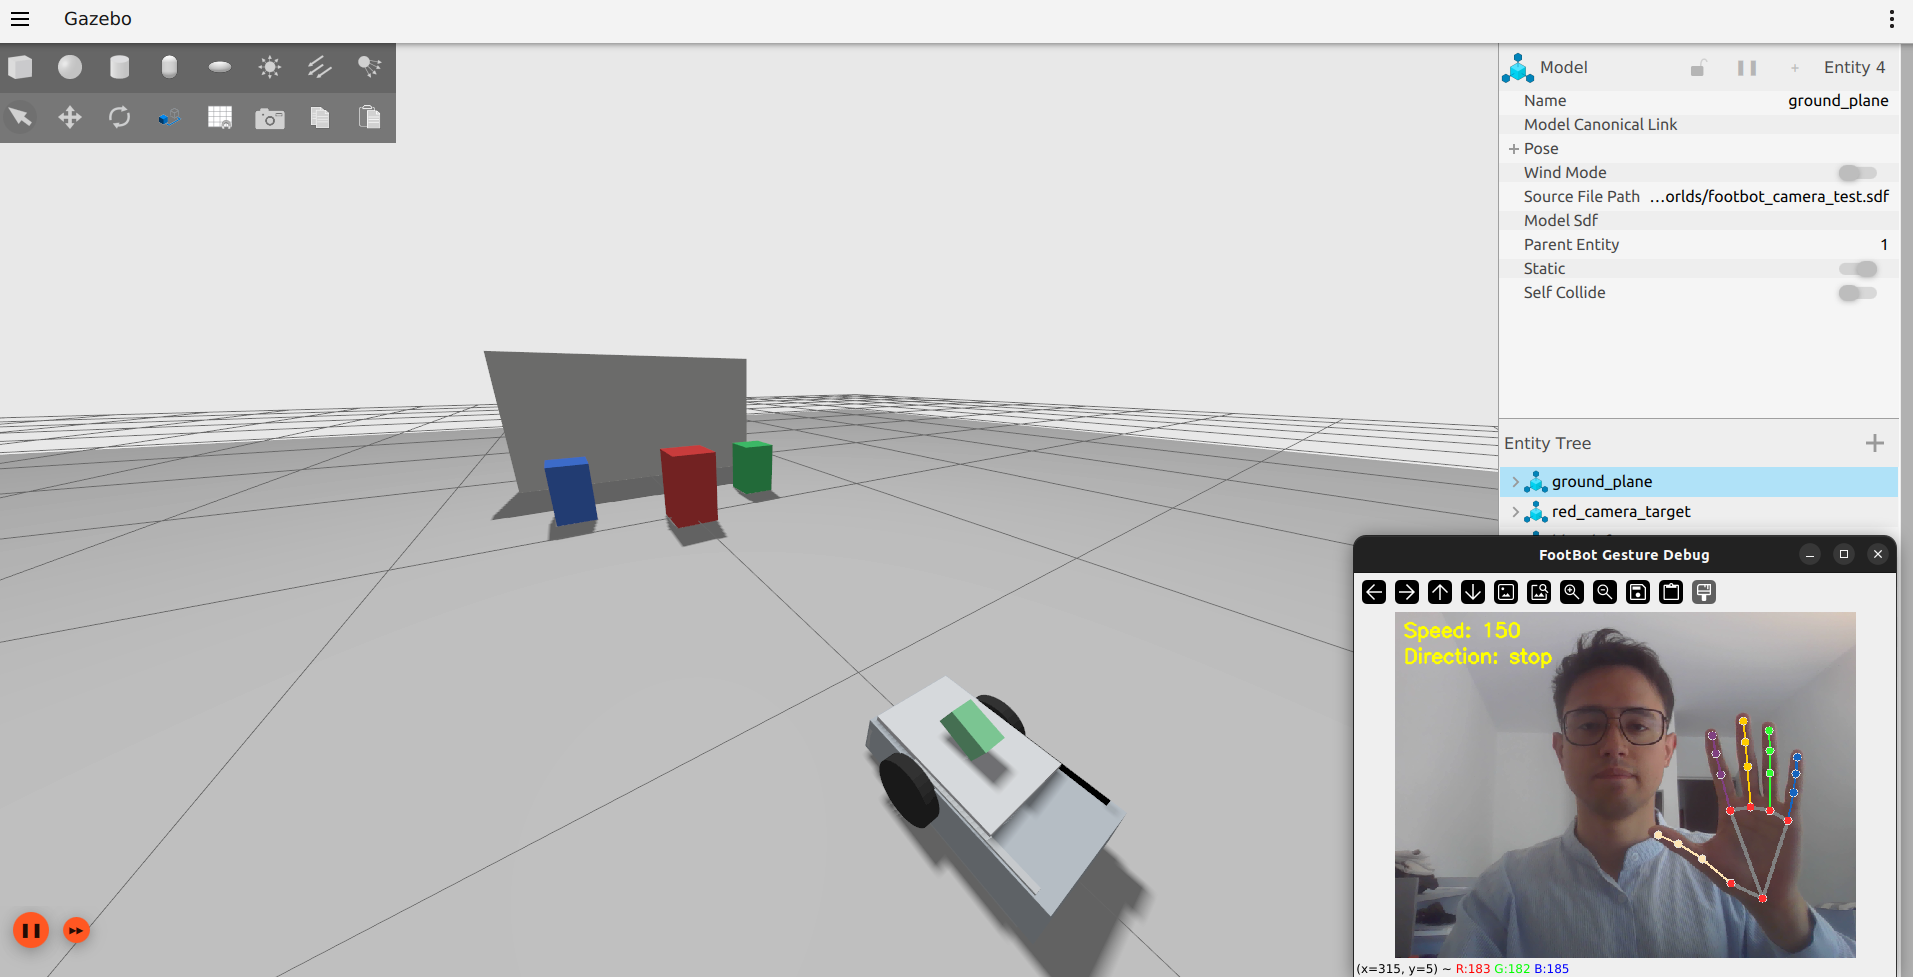
\includegraphics[width=0.74\textwidth]{figures/gesture-debug.png}
\caption{Control por gestos nativo de ROS: vista de depuración con los \emph{landmarks} de la mano de
MediaPipe, la dirección detectada y la realimentación de velocidad.}
\label{fig:gesture}
\end{figure}

\subsection{Tubería de \emph{dataset} y entrenamiento}
Para \emph{Llegar a la portería} se construyó una tubería de datos completa y reproducible:

\begin{enumerate}
  \item \textbf{Captura:} \code{image_capture} guarda imágenes de la escena desde \code{/camera/image_raw}.
  \item \textbf{Etiquetado:} las clases de fútbol (\code{ball}, \code{goal}, \code{opponent}) se etiquetan
  en Label Studio (Fig.~\ref{fig:labeling}) y se exportan en formato YOLO.
  \item \textbf{Aumento:} un script genera copias rotadas/oscurecidas de forma conservadora.
  \item \textbf{Preparación y validación:} se preparan y validan las particiones \code{train}/\code{val}
  del \emph{dataset} de \code{ball} + \code{goal}.
  \item \textbf{Entrenamiento y evaluación:} herramientas de entrenamiento, evaluación y predicción de YOLO
  cierran el ciclo.
\end{enumerate}

\begin{figure}[H]
\centering
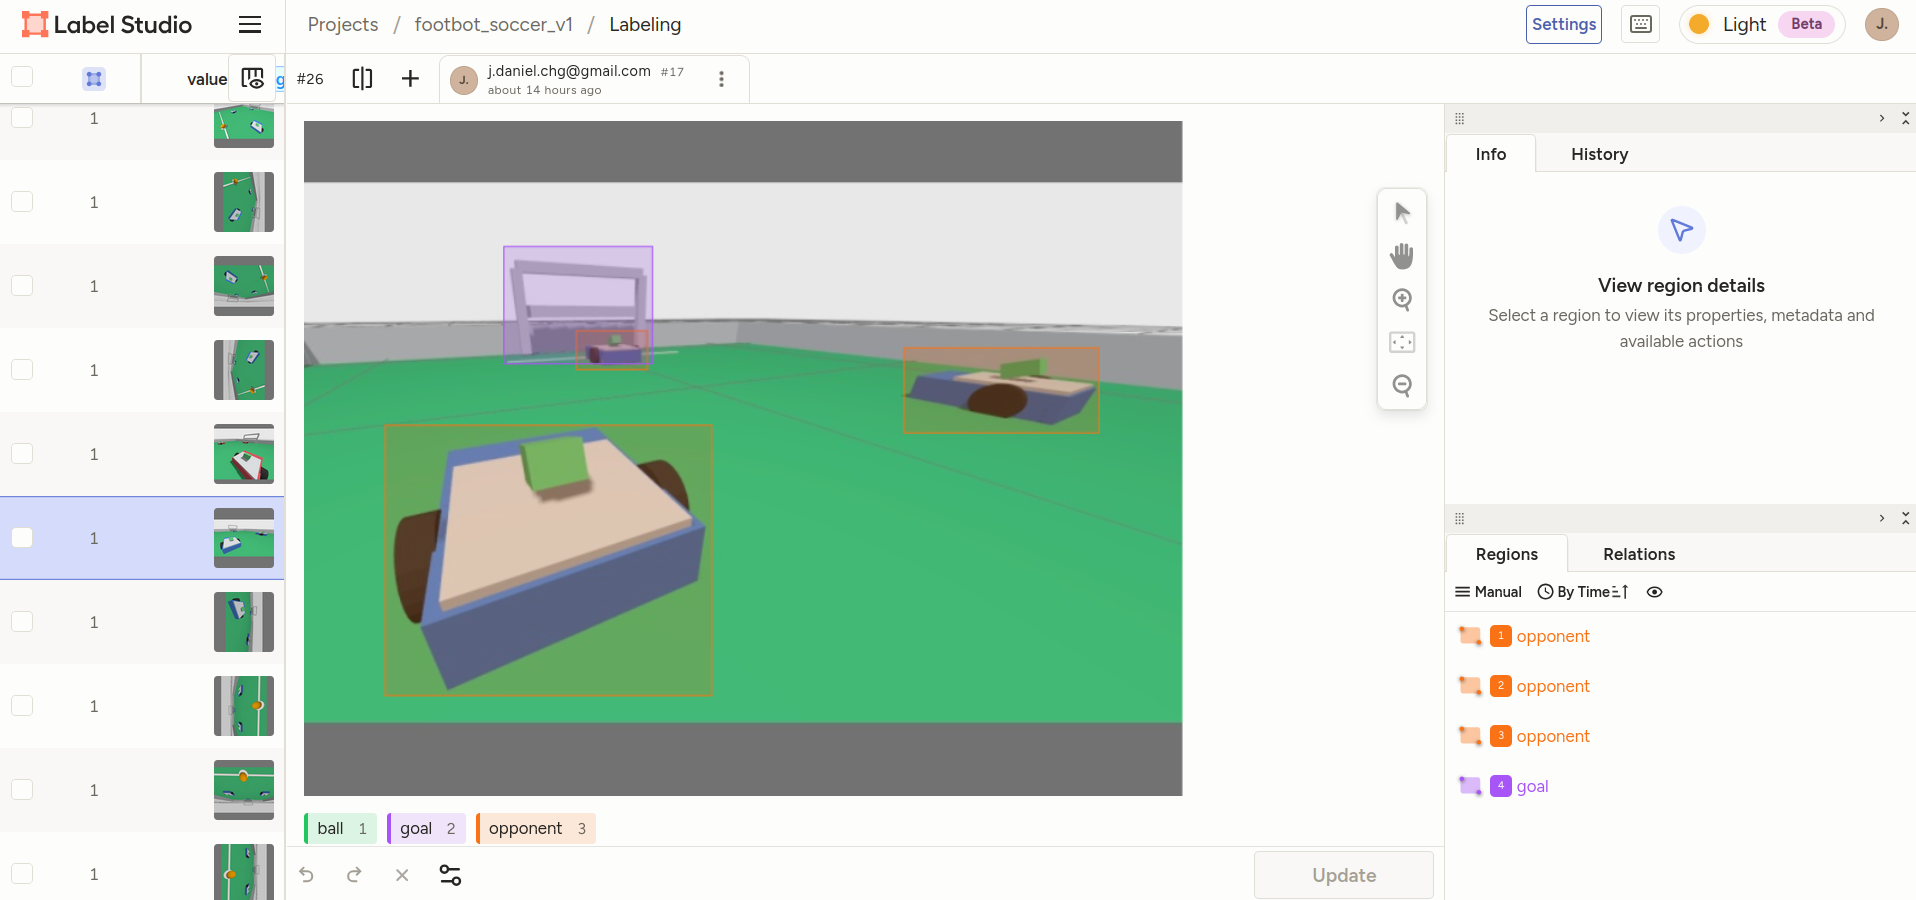
\includegraphics[width=0.74\textwidth]{figures/yolo-labeling.png}
\caption{Etiquetado de objetos de fútbol en Label Studio para el entrenamiento de YOLO, con cajas para
\texttt{ball}, \texttt{goal} y \texttt{opponent}.}
\label{fig:labeling}
\end{figure}

\paragraph{Desempeño del detector.}
Sobre el conjunto de validación, el detector YOLO de \code{ball} y \code{goal} \textbf{funciona muy bien}:
la matriz de confusión del entrenamiento (Fig.~\ref{fig:confmat}) muestra el balón clasificado
correctamente en el 100\,\% de los casos y la portería en el 90\,\% (con un 10\,\% de porterías no
detectadas, confundidas con el fondo). Es decir, \textbf{en las imágenes del \emph{dataset} la percepción
es fiable}. La limitación real no está en el \emph{dataset}, sino \textbf{en despliegue, cuando el robot se
acerca demasiado a la portería}: a corta distancia la portería deja de caber en el cuadro de la cámara y el
detector ya no la reconoce de forma continua, lo que degrada el remate (Sección~\ref{sec:resultados-exp}).

\begin{figure}[H]
\centering
\begin{minipage}[b]{0.49\textwidth}\centering
  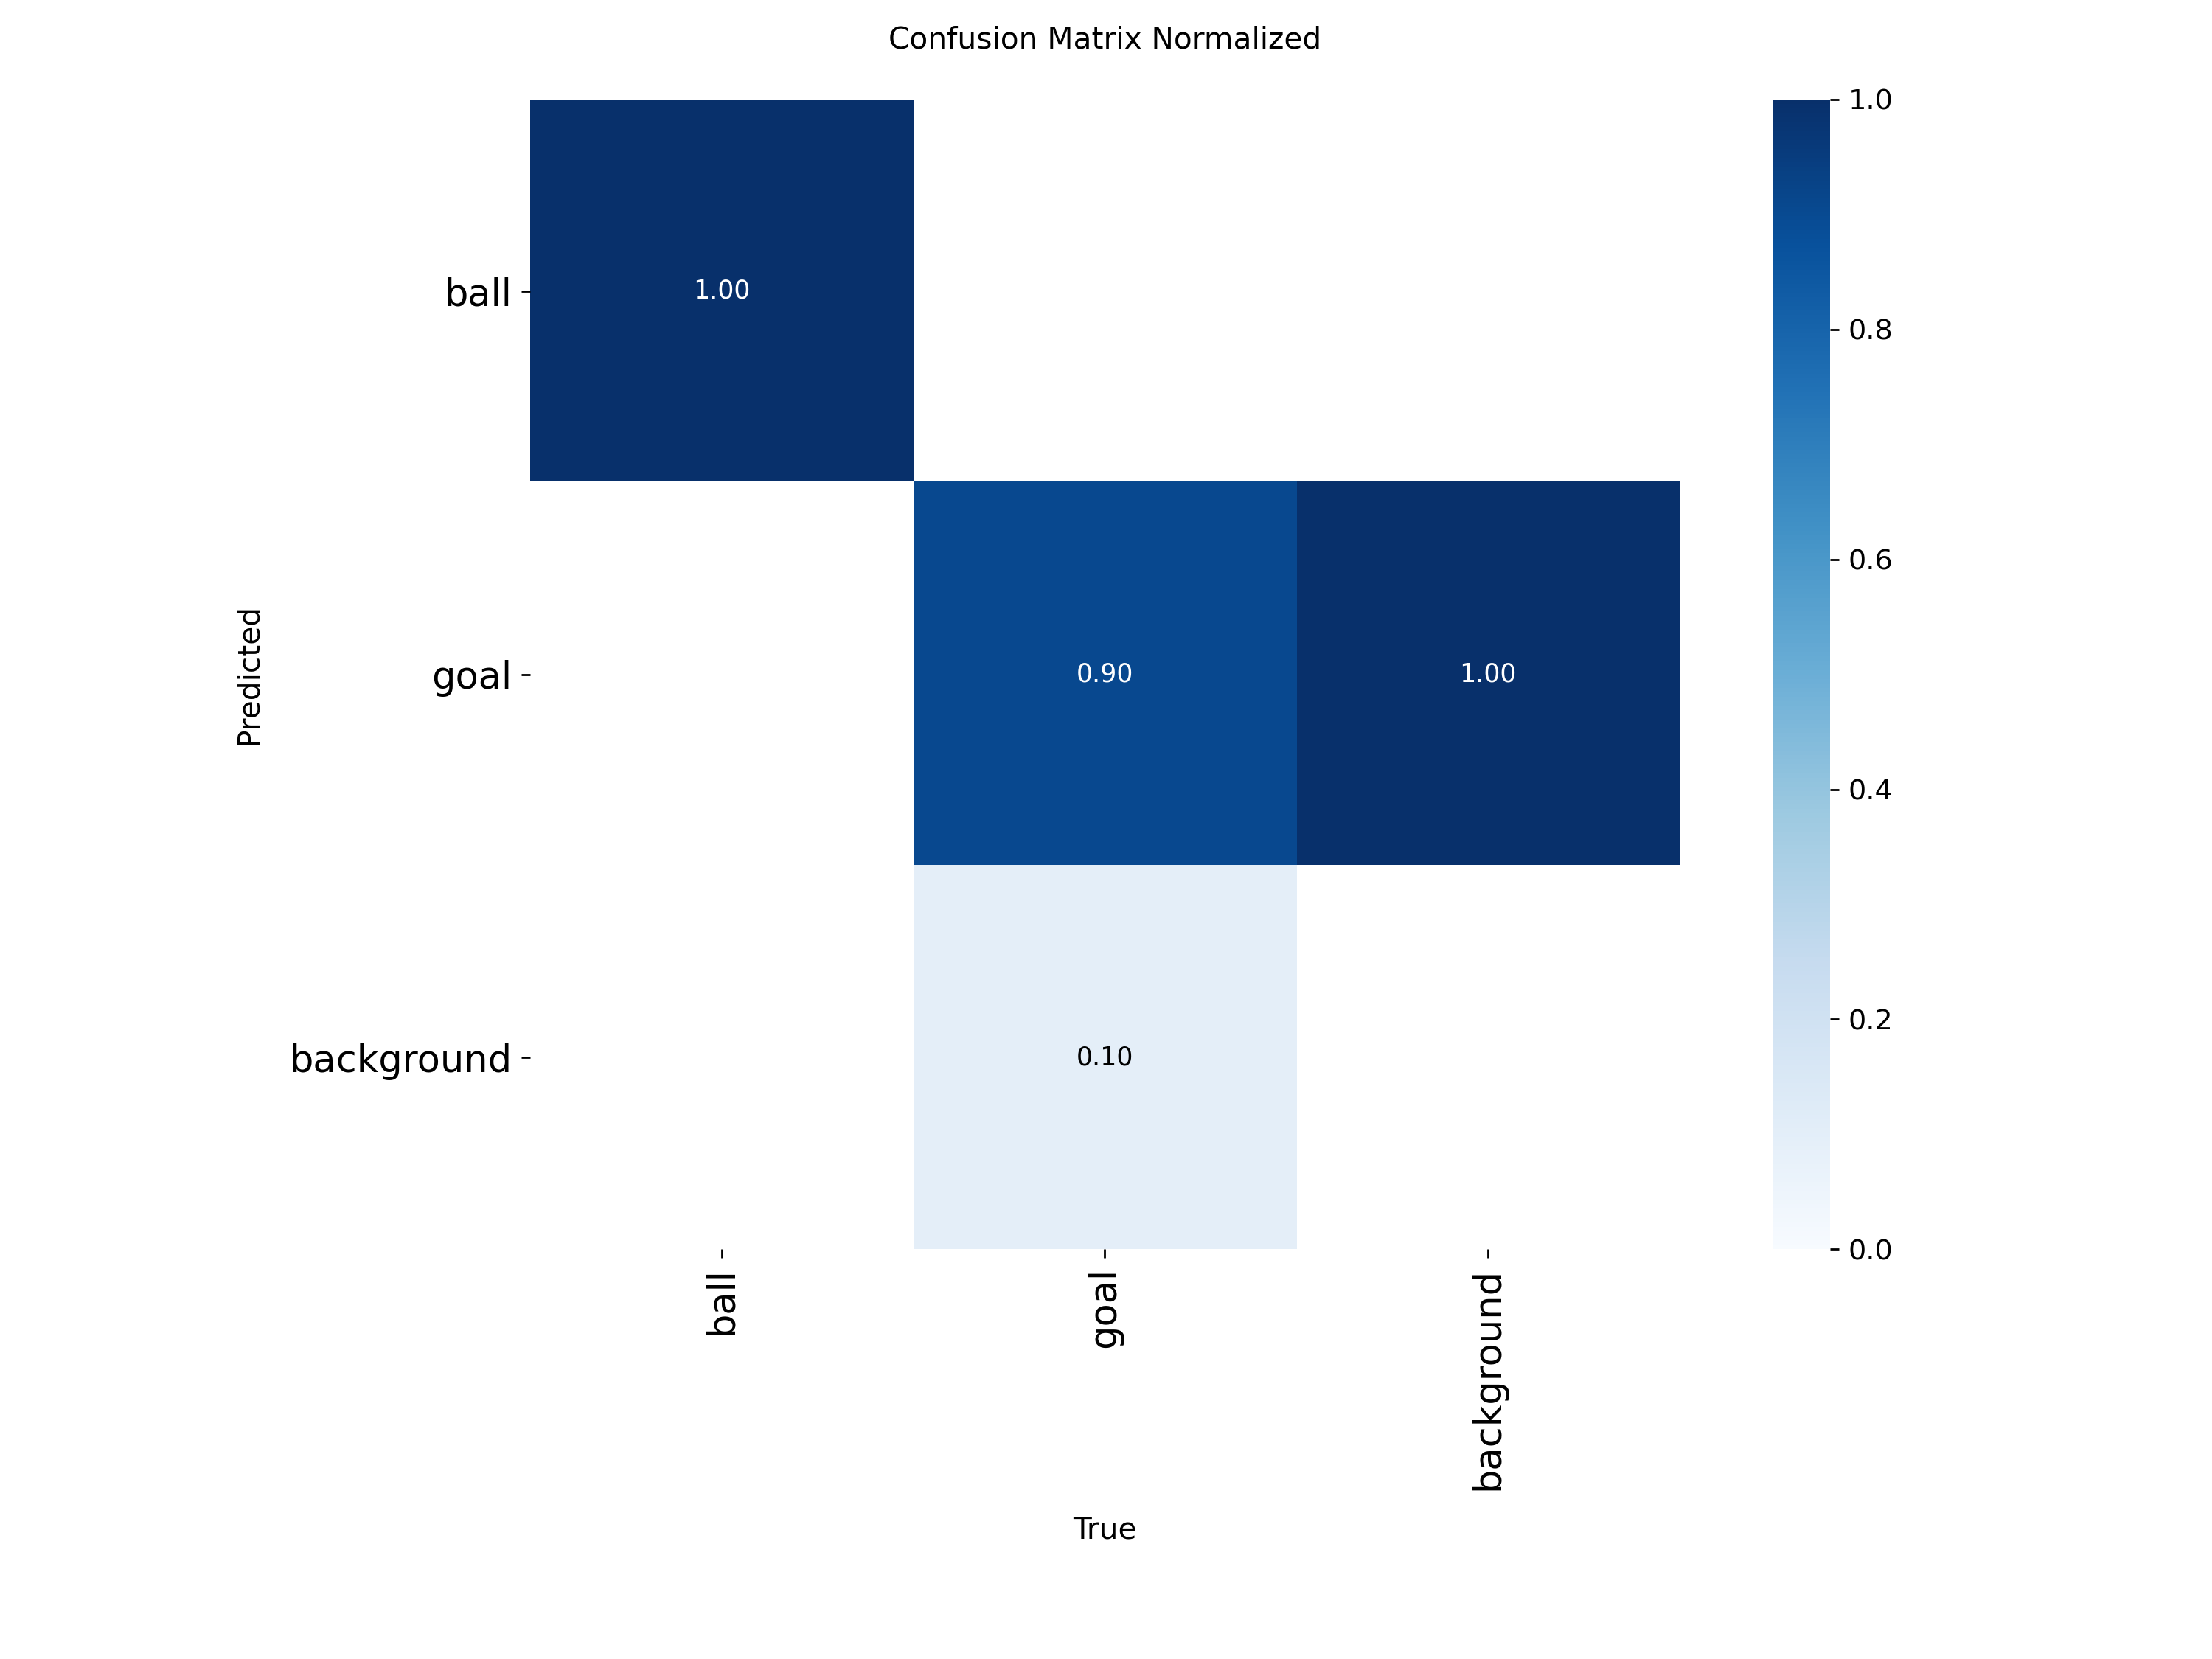
\includegraphics[width=\linewidth]{figures/metrics/yolo_confusion_matrix_normalized.png}\par\smallskip
  {\small (a) Normalizada}
\end{minipage}\hfill
\begin{minipage}[b]{0.49\textwidth}\centering
  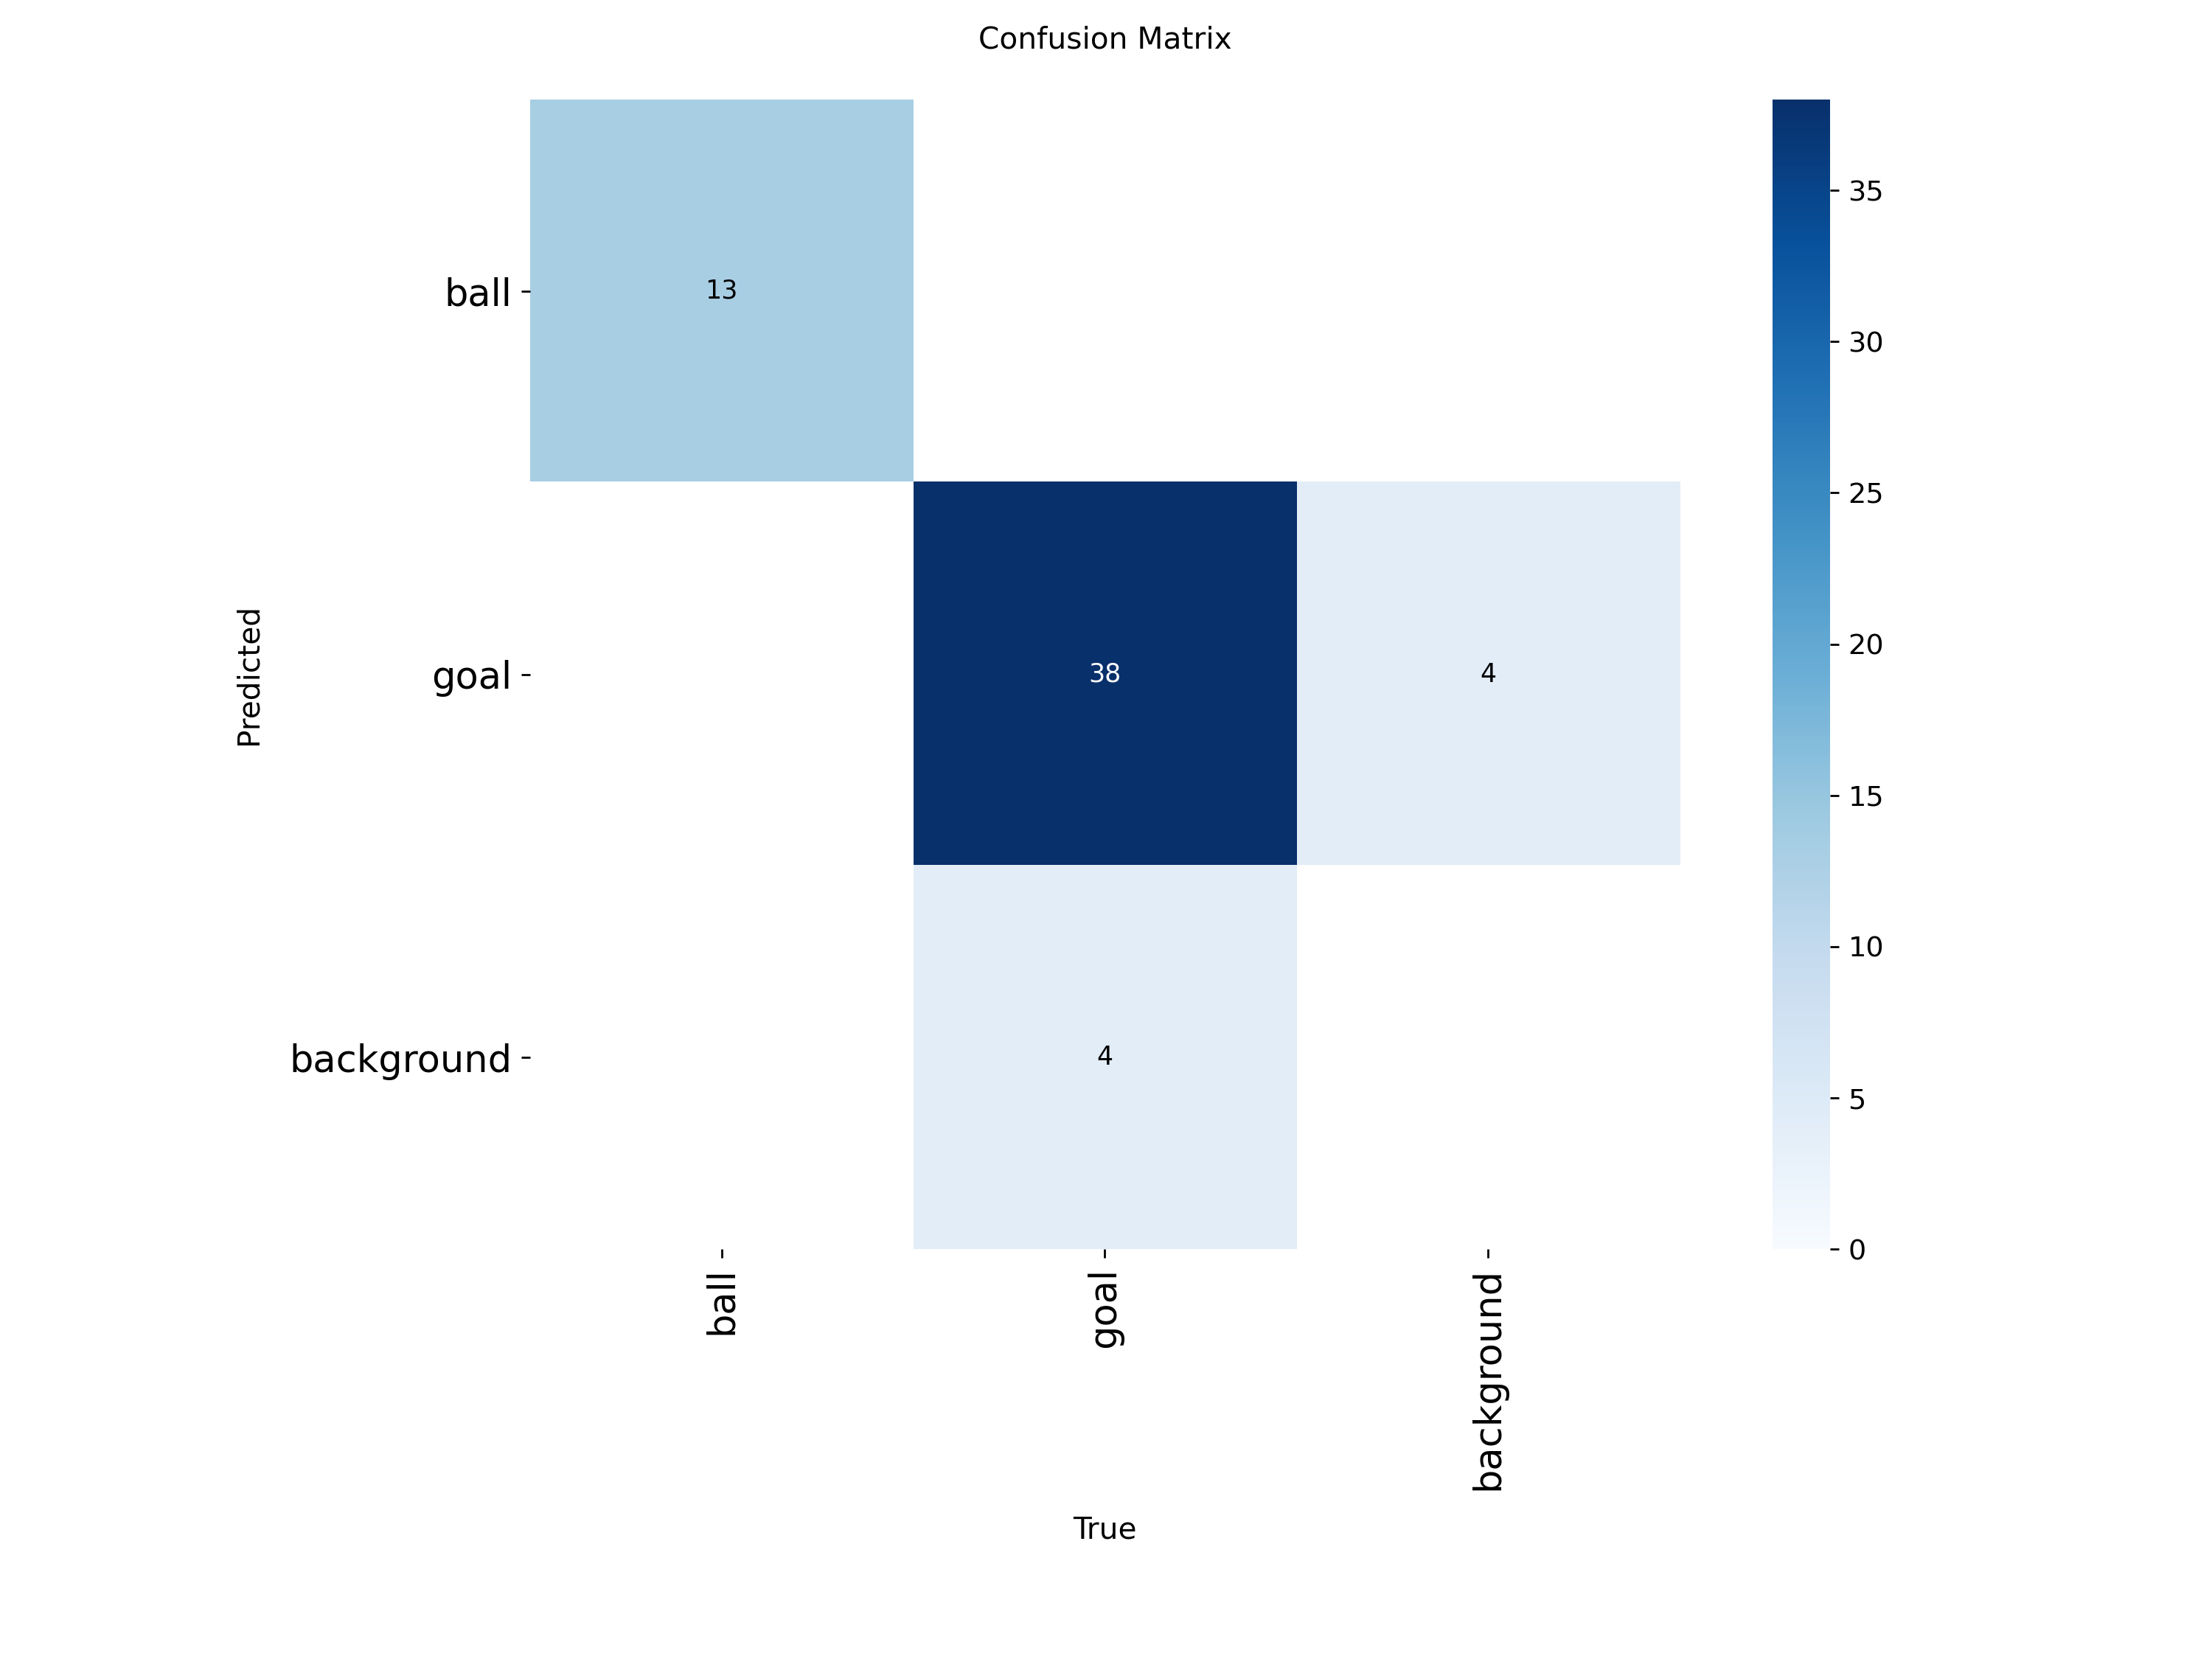
\includegraphics[width=\linewidth]{figures/metrics/yolo_confusion_matrix.png}\par\smallskip
  {\small (b) Conteos absolutos}
\end{minipage}
\caption{Matriz de confusión del entrenamiento de YOLO (\texttt{ball}\,+\,\texttt{goal}) sobre el conjunto
de validación: (a)~normalizada y (b)~en conteos absolutos. El balón se detecta sin error y la portería con
alta fiabilidad en el \emph{dataset}; el problema de detección aparece sólo a muy corta distancia durante
la simulación (Sección~\ref{sec:resultados-exp}).}
\label{fig:confmat}
\end{figure}

% ============================ 8. RESULTADOS ============================
\section{Resultados y estado actual}
\label{sec:resultados}

A la fecha de este reporte, la capa de simulación tiene implementado y funcionando:

\begin{itemize}
  \item Modelo del robot FootBot y generación en Gazebo.
  \item Movimiento por tracción diferencial vía \code{/cmd_vel}.
  \item Puente de compatibilidad HTTP \code{/move} (ESP32) hacia \code{/cmd_vel}.
  \item Cámara simulada del robot y control por gestos nativo de ROS.
  \item Detección HSV del balón y seguidor de balón simple.
  \item \textbf{Control de balón} determinista con orquestación por FSM.
  \item \textbf{Llegar a la portería} determinista, con percepción YOLO de balón\,+\,portería, memoria
  temporal de la portería y un monitor de puntuación de simulación.
  \item Herramientas de \emph{dataset} (validación, preparación, aumento) y de entrenamiento/evaluación de YOLO.
  \item Mundos de campo de fútbol y multi\mbox{-}escenario.
\end{itemize}

\begin{nota}[Verificación]
El \emph{workspace} compila con \emph{colcon} y la suite de pruebas del paquete
\code{footbot_soccer_behavior} pasa correctamente (\textbf{41 pruebas, 0 fallos, 3 omitidas}),
cubriendo la lógica de los estimadores de estado y de las FSM.
\end{nota}

\begin{figure}[H]
\centering
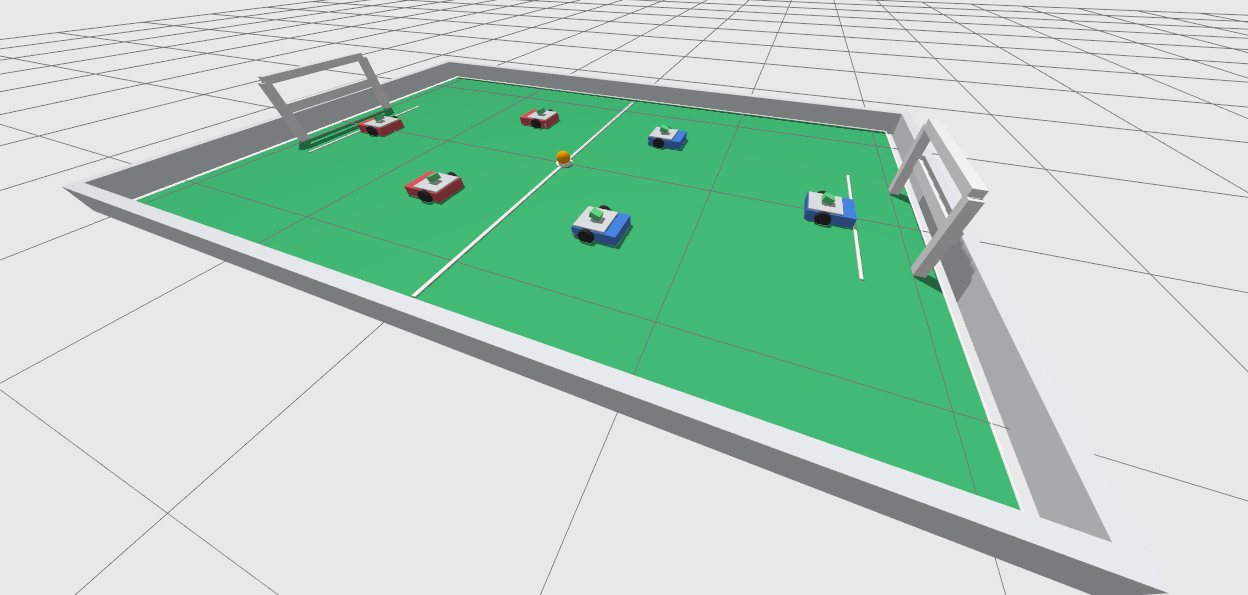
\includegraphics[width=0.80\textwidth]{figures/soccer-field.png}
\caption{Mundo de campo de fútbol completo: paredes de límite, dos porterías, un balón central y
equipos de robots en espejo.}
\label{fig:field}
\end{figure}

\subsection{Análisis experimental: Llegar a la portería (5 episodios)}
\label{sec:resultados-exp}

Se ejecutó una tanda de \textbf{cinco episodios} del comportamiento \emph{Llegar a la portería},
registrando los \emph{topics} con \emph{rosbag2} y procesándolos de forma automática (los \emph{scripts}
de medición y graficado viven en \code{reports/footbot-simulation-es/metrics/}). La
Figura~\ref{fig:reachgoal-exp} muestra una vista cenital del campo —la portería arriba y el robot
partiendo desde abajo— con la trayectoria combinada de los cinco episodios y los mapas de densidad de
permanencia del robot y del balón.

El robot \textbf{controla el balón de forma rápida y consistente} (primer control en $\approx$9~s en
todos los episodios), pero \textbf{rematar resulta costoso}: sólo \textbf{1 de 5} episodios terminó en
gol (20\,\% de éxito) y, en ese caso, tardó cerca de \textbf{269~s}. Tanto las trayectorias como los
mapas de calor muestran que el robot y el balón \textbf{acumulan la mayor parte del tiempo justo frente a
la boca de la portería} (zona superior, en torno a $x\approx1{,}4$~m), sin completar el remate.

\begin{figure}[H]
\centering
\begin{minipage}[b]{0.30\textwidth}\centering
  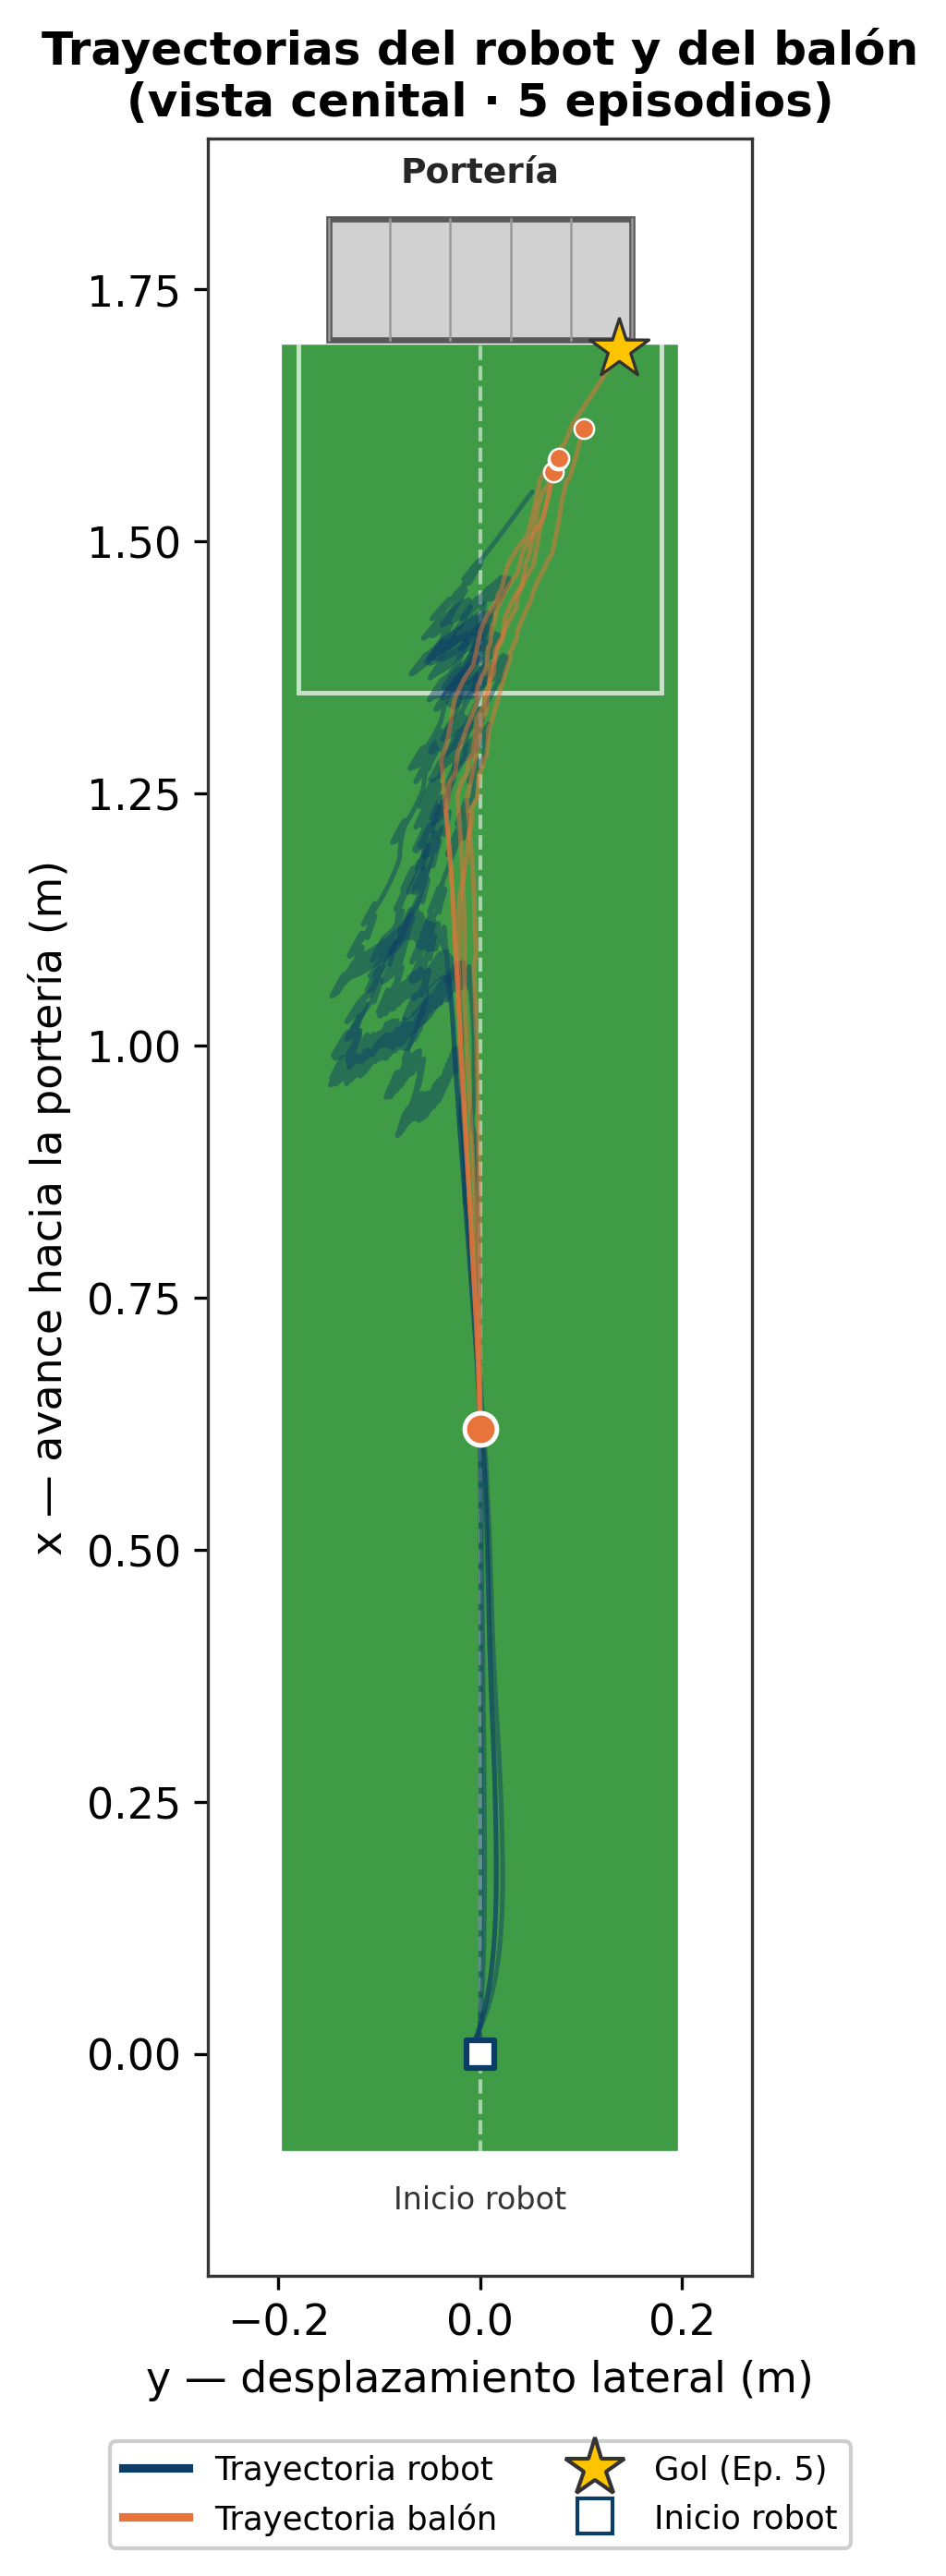
\includegraphics[height=7.8cm]{figures/metrics/trajectory_xy_vertical.png}\par\smallskip
  {\small (a) Trayectorias}
\end{minipage}\hfill
\begin{minipage}[b]{0.33\textwidth}\centering
  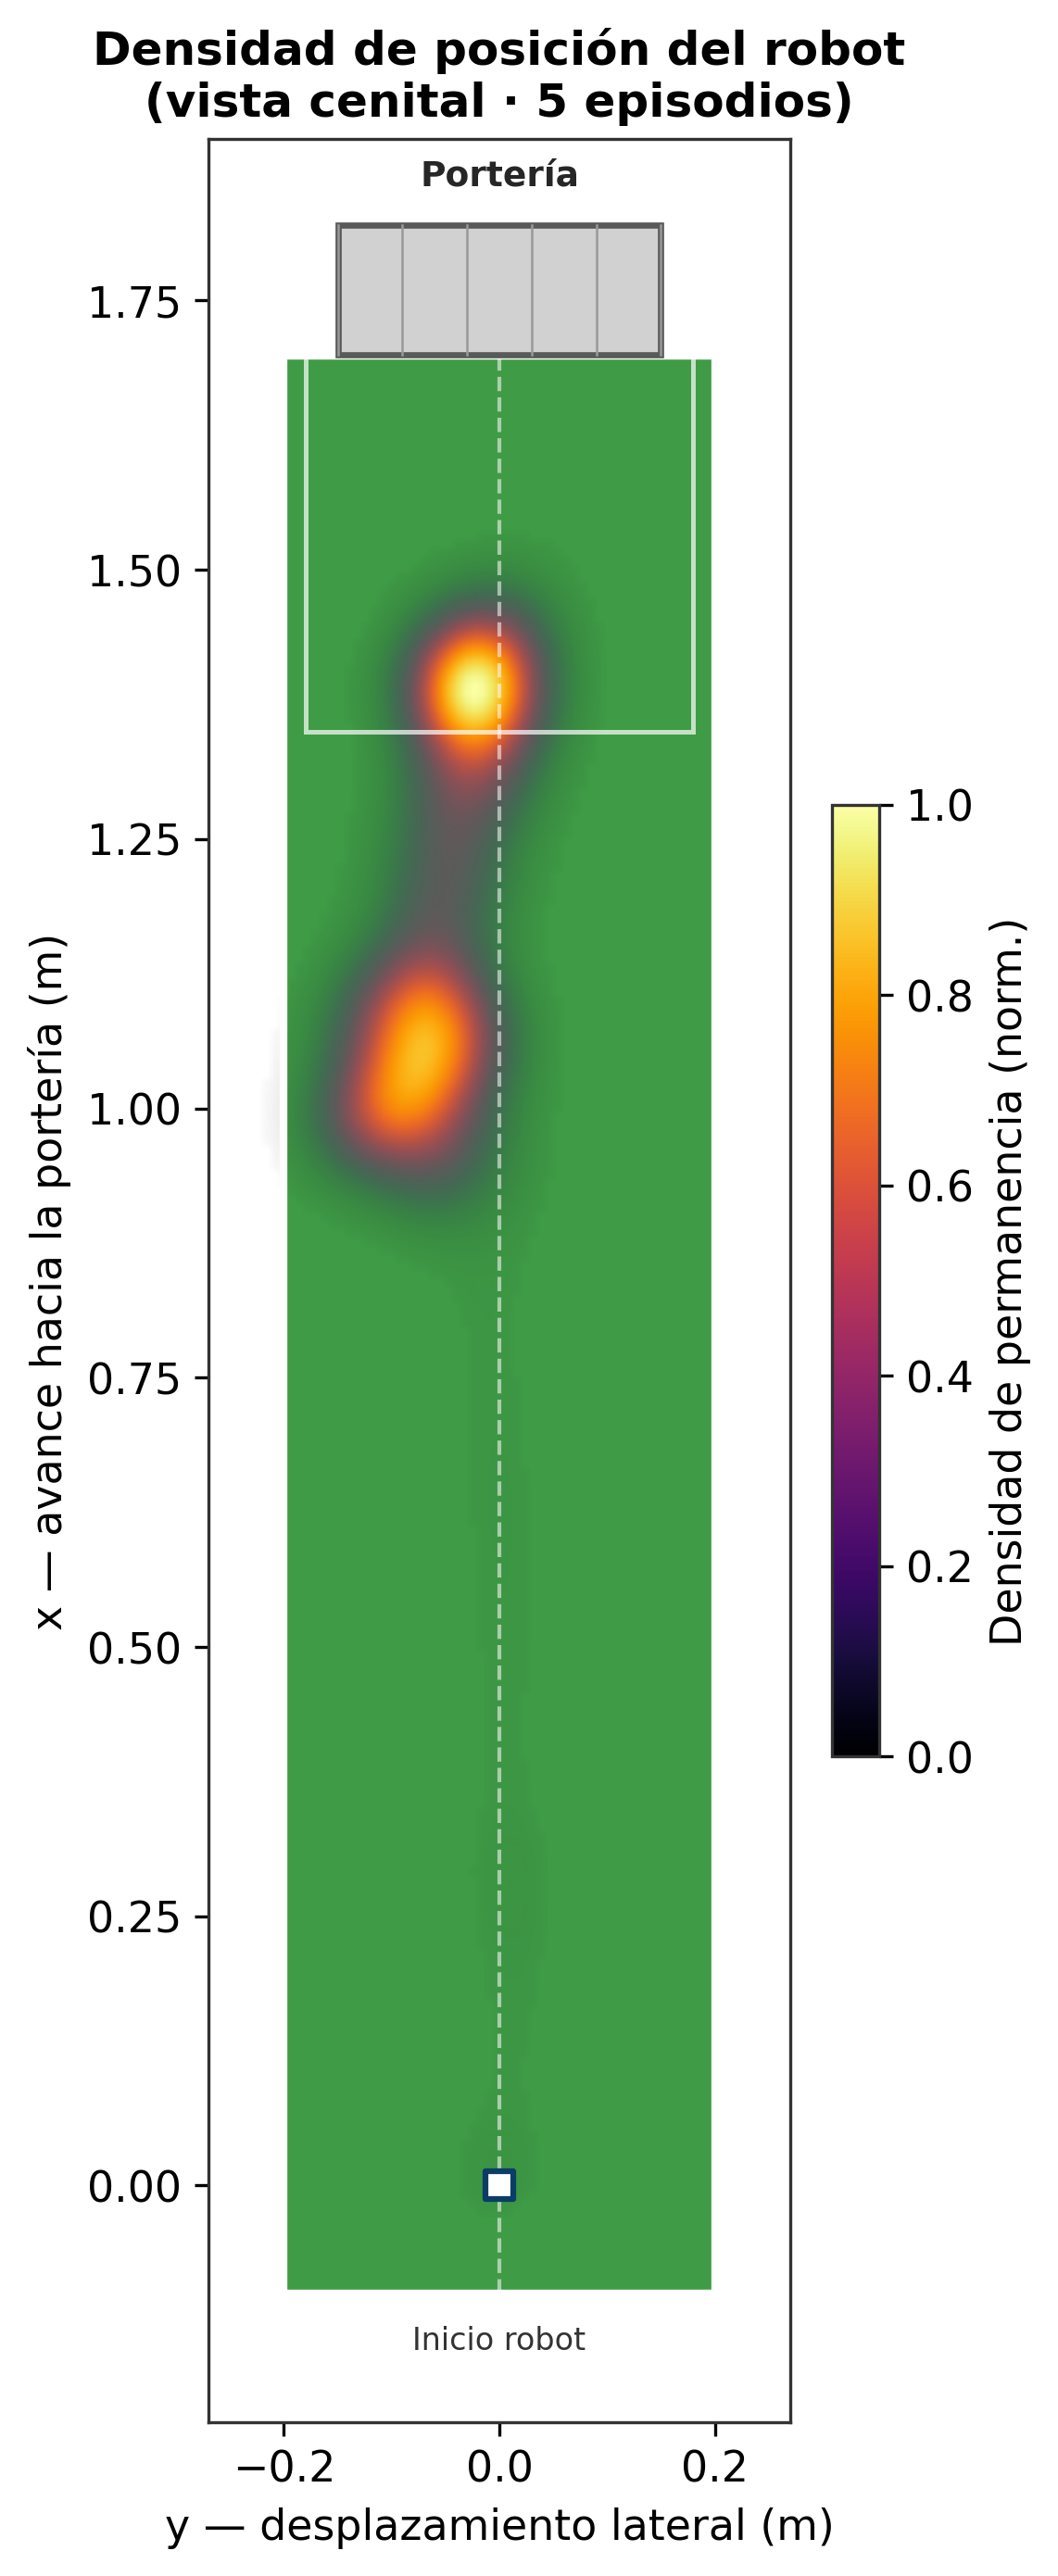
\includegraphics[height=7.8cm]{figures/metrics/robot_heatmap_vertical.png}\par\smallskip
  {\small (b) Densidad — robot}
\end{minipage}\hfill
\begin{minipage}[b]{0.33\textwidth}\centering
  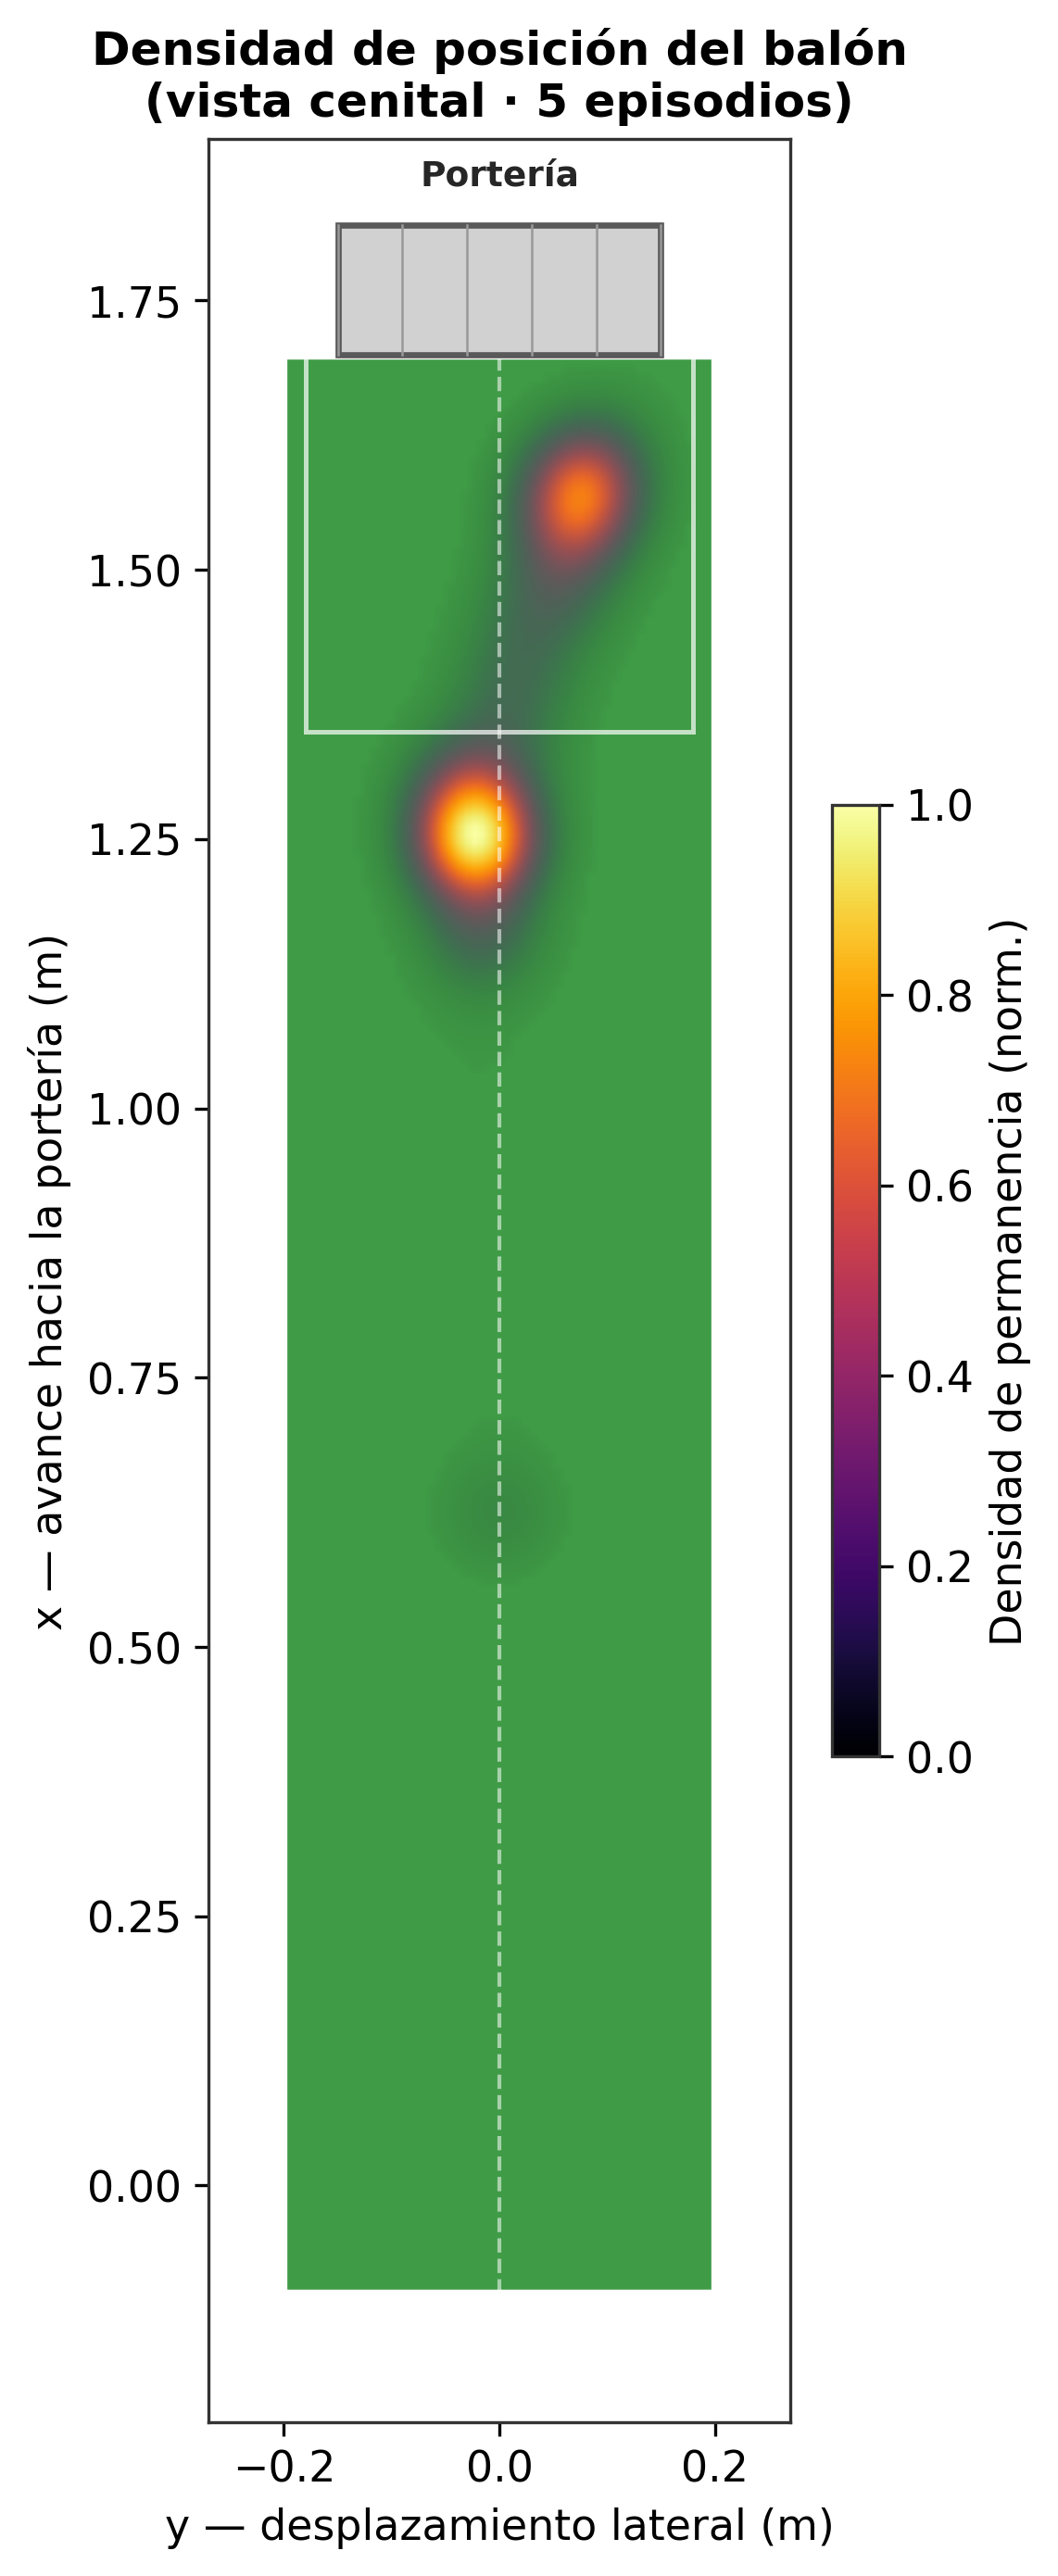
\includegraphics[height=7.8cm]{figures/metrics/ball_heatmap_vertical.png}\par\smallskip
  {\small (c) Densidad — balón}
\end{minipage}
\caption{Análisis cenital de cinco episodios de \emph{Llegar a la portería} (la portería está arriba; el
robot parte desde abajo y avanza hacia ella). (a)~Trayectorias combinadas del robot (azul) y del balón
(naranja); la estrella marca el gol del episodio~5. (b)~Densidad de permanencia del robot y (c)~del balón:
ambos concentran el tiempo \emph{frente a la boca de la portería}, donde la detección visual de la
portería se vuelve intermitente a corta distancia.}
\label{fig:reachgoal-exp}
\end{figure}

\paragraph{Causa principal: detección de la portería a corta distancia.}
El comportamiento se guía por la detección visual de la portería con YOLO. Cuando el robot se
\textbf{acerca mucho}, la portería \textbf{deja de caber por completo en el cuadro de la cámara} y el
detector ya no la reconoce con precisión ni de forma continua: las detecciones se vuelven intermitentes y
la FSM \textbf{pierde la referencia de la portería} repetidamente. En consecuencia, el robot alterna entre
aproximarse, perder el objetivo y \textbf{recuperar/realinear}, lo que dispara el tiempo de remate. La
\emph{memoria temporal de la portería} (Sección~\ref{sec:comportamientos}) atenúa las desapariciones
breves, pero a muy corta distancia no es suficiente.

El \textbf{reparto de tiempo de la FSM} (medido sobre \code{/soccer/reach_goal_fsm_state}) confirma el
patrón: \code{RECOVER_BALL} concentra alrededor del \textbf{33\,\%} del tiempo y \code{APPROACH_BALL} otro
\textbf{26\,\%}, mientras que \code{DRIBBLE_TO_GOAL} —el avance de remate— apenas acumula tiempo. Es decir,
el robot pasa la mayor parte del episodio \emph{recuperando y reaproximándose} en vez de empujar el balón
al fondo. Más revelador aún: el estado de \textbf{respaldo a corta distancia} \code{COMMIT_TO_GOAL}
(Tabla~\ref{tab:reachstates}) —diseñado precisamente para empujar \emph{sin} depender de ver la portería—
\textbf{no se activó en ninguno de los cinco episodios}; el robot siguió dependiendo de la detección
continua de la portería, que es justo lo que falla de cerca.

% ============================ 9. TRABAJO FUTURO ============================
\section{Trabajo futuro}
\label{sec:futuro}

La hoja de ruta mantiene el principio determinista como base estable y añade tácticas sólo cuando son
medibles:

\begin{itemize}
  \item \textbf{Detección de la portería a corta distancia (prioritario):} resolver la pérdida de detección
  cuando el robot está muy cerca y la portería no cabe en el cuadro (Sección~\ref{sec:resultados-exp}).
  Posibles soluciones: (i)~ampliar el \emph{dataset} con vistas de portería a muy corta distancia y
  parciales, y reentrenar YOLO; (ii)~detectar \emph{partes} de la portería (postes, línea de meta) en lugar
  de la caja completa; (iii)~usar una cámara de mayor campo de visión (FOV); (iv)~activar de forma fiable el
  estado de respaldo \code{COMMIT_TO_GOAL} —un \emph{modo de remate por proximidad} que empuja el balón con
  la última pose conocida de la portería y odometría/\emph{dead reckoning}, sin exigir detección continua—;
  y (v)~reforzar la memoria temporal de la portería con anclaje geométrico.
  \item \textbf{Interacción con oponentes:} detectar a un oponente con el balón y disputar la posesión sin
  desestabilizar los comportamientos base; estados de FSM para observar, aproximarse, disputar y recuperar.
  \item \textbf{Juego en equipo:} soportar tres robots por bando con roles (portero, defensor, atacante),
  \emph{namespaces} por robot para evitar colisiones de topics, y comportamiento de pase.
  \item \textbf{Líneas de investigación:} FSM heurísticas y árboles de comportamiento; planificación de
  horizonte corto (MCTS/SPO) y, sólo cuando la simulación tenga \emph{reset}, puntuación y métricas
  estables, aprendizaje por refuerzo (RL/MARL).
\end{itemize}

% ============================ 10. CONCLUSIONES ============================
\section{Conclusiones}
\label{sec:conclusiones}

La migración a ROS\,2 + Gazebo convirtió al FootBot de un banco de pruebas físico, frágil y de iteración
lenta, en un entorno de desarrollo \textbf{reproducible, seguro y escalable}, sin desechar el trabajo previo:
el robot ESP32 y sus aplicaciones siguen como referencia y su protocolo HTTP \code{/move} se conserva mediante
un puente. Sobre esa base se construyeron dos comportamientos de fútbol deterministas —Control de balón y
Llegar a la portería— bajo un patrón claro de \emph{percepción $\rightarrow$ estado $\rightarrow$ FSM $\rightarrow$
un único dueño de} \code{/cmd_vel}, junto con una tubería completa de \emph{datasets} y entrenamiento de visión.
El resultado es una plataforma sólida para las siguientes etapas: oponentes, juego en equipo y experimentos
tácticos.

% ============================ REFERENCIAS ============================
\section*{Referencias}
\addcontentsline{toc}{section}{Referencias}
\begin{itemize}[leftmargin=1.4em]
  \item Documentación técnica del proyecto: \code{simulation/docs/} (índice, arquitectura, modos,
  control de balón, llegar a la portería, percepción y \emph{datasets}, mundos y escenarios).
  \item ROS\,2 Humble — Instalación en Ubuntu: \url{https://docs.ros.org/en/humble/Installation/Ubuntu-Install-Debs.html}
  \item Gazebo Fortress — Documentación: \url{https://gazebosim.org/docs/fortress/install}
  \item Ultralytics YOLO: \url{https://github.com/ultralytics/ultralytics}
  \item MediaPipe (Google): \url{https://github.com/google/mediapipe}
\end{itemize}

\end{document}
